\documentclass[titlepage]{article}

\usepackage{graphicx}
\usepackage{longtable}
\usepackage{float}
\usepackage{subfig}
\usepackage{enumitem}
\usepackage{hyperref} 
\usepackage{tasks}
\graphicspath{ {./images/} }


\title{{\Huge {\it {\it Data4Help}}}}
\author{Lorenzo, Molteni, Negri}
\date{January 13, 2019}

\begin{document}
	
	\makeatletter
	\begin{titlepage}
		\begin{center}
			
\includegraphics[width=\linewidth]{logo.png}\\[20ex]
			{\huge  \@title }\\[2ex] 
			{\LARGE  \@author}\\[3ex] 
			{\LARGE {\it ITD} - Implementation \& Testing Document}\\[3ex]
			{\large \@date}\\[5ex]
		\end{center}
	\end{titlepage}
	\makeatother
	\thispagestyle{empty}
	\newpage
	
	%Add content for page two here (useful for two-sided printing)
	\thispagestyle{empty}
	\newpage
	
	
	
	%Index	
	\pagebreak
	\tableofcontents{}
	\pagebreak
	
	
	%Introduction
	\section{Introduction}
	\subsection{Purpose and Scope}
	This Document contains a detailed and exhaustive explanation of the implementation of the {\it Data4Help} project. The purpose of this document is to explicitly detail the rationale of all choices made and provide a complete overview of how the project source code is structured and designed.
	The document also tackles the software testing activities and shows what are the main tests that have been performed on the product.
	
	\subsection{Definitions, Acronyms, Abbreviations}
	\subsubsection{Definitions}
	\begin{itemize}
		\item {\bf Framework}
		a software framework can be defined as a standard way to build and deploy applications. It is a universal, reusable software environment that provides particular functionality as part of a larger software platform to facilitate development of software applications, products and solutions. Software frameworks include compilers, code libraries, tool sets, and application programming interfaces (APIs).
		
		\item {\bf Library}
		a software library is a set of pre-written pieces of code: classes, algorithms, structures and procedures that implement standard functionalities saving developers the time to implement them from scratch. It is important to point out the difference between libraries and frameworks. While libraries\textsc{\char13} functions are explicitly called by the programmer when they are needed, a frameworks makes programming faster by setting some constraints on how the project is structured and organised.
		
		\item {\bf Package Manager}
		a package manager is a software tool that automates the process of installing, upgrading, configuring, and removing libraries. A package manager in particular deals with software dependencies and versions and prevents software mismatches and missing prerequisites. In this project two different package managers have been used: CocoaPods to help the development of the XCode project for the front-end and NPM, Node Package Manager, to deal with the back-end dependencies.
	\end{itemize}
	\subsubsection{Acronyms}
	\renewcommand*{\arraystretch}{1.4}
	\begin{longtable}{| p{2 cm} | p{7 cm} |} \hline
		{\bf DBMS} & Data Base Management System \\ \hline
		{\bf REST} & REpresentational State Transfer \\ \hline
		{\bf API} & Application Programming Interface \\ \hline
		{\bf OS} & Operating System\\ \hline
		{\bf UI} & User Interface \\ \hline
		{\bf HTTP} & HyperText Transfer Protocol \\ \hline	
		{\bf URL} & Uniform Resource Locator \\ \hline
		{\bf JSON} & JavaScript Object Notation \\ \hline
		{\bf DB} & Database \\ \hline
		{\bf AWS} & Amazon Web Services \\ \hline
		\caption{Acronyms}	
		
	\end{longtable}
	\subsubsection{Abbreviations}
	
	\begin{itemize}
		\item {\bf (Rn):} n-th Requirement
	\end{itemize}
	
	\subsection{Reference Documents}
	\begin{itemize}
		\item {RASD Document}
		\item {Design Document}
		\item {Implementation and Testing project assignment}
		\item {The Swift Programming Language (Swift 4.2)}
		\item {The Criteria Committee of the New York Heart Association. Nomenclature and Criteria for Diagnosis of Diseases of the Heart and Great Vessels. 9th ed. Boston, Mass: Little, Brown \& Co; 1994:253-256.}
	\end{itemize}
	
	\subsection{Overview}
	The remaining parts of the implementation document are organised as follows:
	\begin{itemize}
		\item {\bf Requirements implemented:}
		shows the functions that are actually implemented in the software and how they are mapped on the requirements identified in the RASD document.
		
		\item {\bf Design choices and adopted Frameworks:}
		lists all the adopted programming languages, middlewares and frameworks adopted and provides their advantages and disadvantages. It also shows the reasons behind the implementations decisions made to follow the solution identified in the Design Document.
		
		\item {\bf Source code structure:}
		explains how the source code is structured and organised for both the front-end and the back-end.
		
		\item {\bf Testing:}
		provides information on how testing has been performed. In particular it describes the procedures followed and the main test cases that has been considered as well as their outcome.
		
		\item{\bf Future development:}
		lists all non implemented functionalities and provides a description of future releases
		
		\item {\bf Installation:}
		contains all the information needed to install and run the software.
	\end{itemize}
	
	
	\pagebreak
	%%%%%%%%%%%%%%%%%%%%%%%%%%%%%%%%%%%%%%%%%%%%%%%%%%%%%%%%%%%%%%%%%%%%%%%%%%%%%%%%%%%%%
	%Requirements Implemented
	\section{Requirements Implemented}
	\begin{itemize}
		\item {\bf [R1]} The S2B allows users to create either a {\it Single User} or a {\it Third Party} account. 
		\item {\bf [R5]} To access the service users must log in with their account credentials.
	\end{itemize}	
	
	\subsection{User Authentication}
	\begin{itemize}
		\item R1 The S2B allows users to create either a Single User or a Third Party account.
		\item R5 To access the service users must log in with their account cre- dentials.
	\end{itemize}
	
	{\bf Database} \newline
	To access {\it Data4Help}\textsc{\char13}s services a user will be asked to register to the service. Information concerning registration is stored in our database in the Registration table. Each row in the table uniquely identifies a user through its userID and stores a boolean value saying whether the account has been activated or not. After registration, each login session will be identified by a token that will be bound to the user\textsc{\char13}s ID until logout.
	\newline
	\newline
	\noindent
	{\bf Frontend} \newline
	The client application performs an automatic login if some user credentials are already stored in the {\it System}. Otherwise the user will be brought to the login view, which present an undifferentiated form to fill (username, password) in order to access the {\it System} either as a {\it Single User} or as a {\it Third Party}. When the user clicks on the login button the application checks whether all fields have been filled and proceeds to send a HTTP POST request to the backend. In case of positive response the application uses the content of the response message to determine whether the logged user is a {\it Single User} or a {\it Third Party} and to consequently perform a segue to the appropriate view. For what concerns the registration of new users,  the {\it System} provides differents views for {\it Single User} and {\it Third Parties}, each with the appropriate form fields to fill. If after clicking the registration button a positive response is received the applications goes back to the login view. The user, after activating its account from the email, will be able to log in.   
	\newline
	\newline
	\noindent
	{\bf Backend} \newline
	Authentication is managed by the /req/auth endpoints, offering registration for a {\it Single User} and for a {\it Third Party}, account activation and login. 
	When registering, the database is queried to find out whether the provided data is already associated to another account; if not, a unique userID is generated, and an activation token is sent by email to the address using to register.
	When the user activates its account, if the token is valid, the database is updated to complete the creation process. Then, whenever the user logins with correct credentials, a secure token is generated using JWT (HS256 encryption), storing the id of the user and the type of account ({\it Single User} or {\it Third Party}) as its content.
	
	
	\subsection{User Management}
	\begin{itemize}
		\item {\bf [R1]} The S2B allows users to create either a {\it Single User} or a {\it Third Party} account. 
		\item {\bf [R2]} A {\it Single User} account can be created if and only if the user provides his Fiscal Code. 
		\item {\bf [R3]} A {\it Third Party} account can be created if and only if a valid P.IVA is provided. 
		\item {\bf [R4]} All users can create an account if and only if they provide a unique email and a password. 
		\item {\bf [R5]} To access the service users must log in with their account credentials.
		\item {\bf [R35]} The S2B allows organisers to create a {\it Third Party} account using {\it Data4Help}.
		\item {\bf [R43]} The S2B allows runners to create a {\it Single User} account using {\it Data4Help}.
	\end{itemize}			
	
	{\bf Database} \newline
	According to the type of account created, all information concerning a user will be stored in either the PrivateUser table or the ThirdPartyUser table. In both tables users are uniquely identified by a userID and an email. Both will be associated with a properly hashed password. The table concerning {\it Single User} data will also store the user\textsc{\char13}s FC, if available, its name, birthday and sex. That concerning {\it Third Parties} instead will store the company\textsc{\char13}s name, P.IVA and description. 
	Finally, the UserSettings table uniquely concerns {\it Single User} accounts and stores information about which types of health data to import from their device. When imported, all health data concerning a user is stored in the UserData table. Each record is identified by the user\textsc{\char13}s userID, its type, its timestamp and stores the measured value.
	\newline
	\newline
	\noindent
	{\bf Frontend} \newline
	When the user opens the app for the first time he will be asked what kind of health data he is willing to import into {\it Data4Help}\textsc{\char13}s {\it System}. User credentials and information are set during registration phase and following the thin client paradigm there is no persistent user model, but all data (shown in the settings tab) are retrieved with a HTTP GET request to the backend. Both {\it Third Parties} and {\it Single Users} can modify some of their information at any time from the Settings tab. Some critical information cannot be changed after registration. These include: email, FC, P.IVA. 
	\newline
	\newline
	\noindent
	{\bf Backend} \newline
	For settings management, two endpoints are offered: /single/info and /tp/info, respectively for {\it Single Users} and {\it Third Parties}. When sending a GET request to those endpoints, the server queries the database to retrieve the settings of the user that can be modified, thus not including password and sex, for example. When the request received is a POST, the body will contain the fields that the user wants to update, so the database will be queried to save these new settings.
	
	
	\subsection{Creation of Single Requests}
	\begin{itemize}
		\item {\bf [R9]} Third Parties can submit a request to access data of a {\it Single User}. 
		\item {\bf [R10]} Single Requests must specify either the email or the FC of the desired user.
		\item {\bf [R11]} Single Requests are forwarded only to the specified user.
		\item {\bf [R12]} A user can accept or refuse requests forwarded to him. 
		\item {\bf [R13]} Third Parties can access user\textsc{\char13}s data if and only if their request is accepted by said user. 
		\item {\bf [R17]} Single requests must specify the requested data types. 
		\item {\bf [R18]} A request to a {\it Single User} must specify whether or not the {\it Third Party} is subscribing to that request of data.
		\item {\bf [R19]} Subscriptions to requests must specify a duration.
		\item {\bf [R20]} Subscriptions to requests can be ended by both the {\it Third Party} and the {\it Single User} at any time.
		\item {\bf [R21]} If none of the requested data types of the {\it Single User} is available, the {\it Third Party} receives an error message.
		\item {\bf [R22]} Third Parties can access only the requested data types that are available.
		\item {\bf [R23]} Third Parties can download all data obtained through requests on their devices or have it sent by email.
		\item {\bf [R39]} The request is sent on behalf of the organiser using its email and P.IVA.
		\item {\bf [R40]} The request sent is with a subscription that lasts until the end of the run.
		\item {\bf [R41]} The request sent by the S2B has as requested data types the position and all available health parameters of the user.
		\item {\bf [R47]} A user can\textsc{\char13}t accept the request if he doesn\textsc{\char13}t have at least his position available as requestable data type.
	\end{itemize}	
	
	
	{\bf Database} \newline
	When a {\it Third Party} creates a Single Request, all its related information is stored in the SingleRequest table. Each request is uniquely identified by a requestID and specifies its {\it Third Party} sender, {\it Single User} receiver, its status and specification on whether it is a subscription or not. The content of each request must be stored in the RequestContent table. The content includes the request\textsc{\char13}s unique ID and the requested type of health data.
	Each Single Request addresses a {\it Single User} that is able to accept it or refuse it. The information on the status of the request is stored in the SingleRequest table under the field status that is initially pending and is modified to accepted or refused according to the {\it Single User}\textsc{\char13}s action. The various statuses are described by the requeststatus enumeration.
	\newline
	\newline
	\noindent
	{\bf Frontend} \newline
	{\it Third Parties} can send single requests from the associated view in the Research tab. The view contains a form to be filled with either FC or email to identify the {\it Single User}, and a serie of toggles to specify what kind of data are requested. After the “Send request” button is pressed an HTTP POST request containing all the information is sent to the backend.
	{\it Single Users} can see all the request pertaining to them in the “MyFollowers” tab and can accept or refuse pending requests by tapping on some buttons. {\it Third Parties} can see a list of all the Single Requests they send in the “MyHistory” tab and they are able to either stop the eventual subscription prematurely or download a csv file containing all the data related to a certain Group Request. 
	\newline
	\newline
	\noindent
	{\bf Backend} \newline
	For {\it Third Parties}, the server offers the /tp/sendSingle endpoint to create and send a request to the target user. To be able to send it, there shouldn\textsc{\char13}t be another pending request from the {\it Third Party} to the {\it Single User}. If this condition is met, then the request is inserted in the DB. {\it Third Parties} can then download the results of a request by sending a POST to /tp/downloadSingle, but only if such request (identified by its unique id) was approved, in this case data is retrieved from the database up until the date of the request, or the end of the subscription (if present).
	{\it Single Users} can accept or refuse a request they received through the /single/choice endpoint, and also terminate an ongoing subscription through the /sub/endSingle endpoint. To retrieve the list of requests meant for them, {\it Single Users} can query the /single/list endpoint.
	
	
	\subsection{Creation of Group Requests}
	\begin{itemize}
		\item {\bf [R19]} Subscriptions to requests must specify a duration.
		\item {\bf [R23]} Third Parties can download all data obtained through requests on their devices or have it sent by email.
		\item {\bf [R26]} Third Parties can submit a group request to access data of groups of users. 
		\item {\bf [R25]} Group requests must include at least one search parameter.
		\item {\bf [R26]} Group requests must specify the requested data types. 
		\item {\bf [R27]} Group request results are provided if and only if the number of users matching the search parameters is higher than 1000. 
		\item {\bf [R28]} Group request results include only the data retrieved by the {\it System} matching the search parameters. 
		\item {\bf [R30]} All group requests must specify whether the {\it Third Party} is subscribing to that request of data. 
		\item {\bf [R31]} Subscriptions to requests can be ended by the {\it Third Party} at any time.
	\end{itemize}	
	
	{\bf Database} \newline
	All information concerning group requests created by {\it Third Parties} is stored in the GroupRequest table. This keeps track of all requests identified by a unique requestID and specifying the {\it Third Party} sender, the request status and information concerning the subscription. Furthermore each group request may be associated to one or more tuples in the SearchParameters table. This stores all filters for group requests by associating a requestID to a type of health data, its requested lower and upper bounds.
	All group requests have initially set the field status to pending. However, once they are evaluated, the field is then set to either accepted or refused according to the evaluation of the filters on users.
	\newline
	\newline
	\noindent
	{\bf Frontend} \newline
	{\it Third Parties} can send group requests from the associated view in the Research tab. The view contains a serie of toggles to select the requested data and a number of sliders and text fields to specify the filtering parameters for the request. After the “Send request” button is pressed an HTTP POST request containing all the information is sent to the backend.
	{\it Third Parties} can see the list of all the Group Requests they sent in the “MyHistory” tab and they are able to either stop the eventual subscription prematurely or download a csv file containing all the data related to a certain Group Request. 
	\newline
	\newline
	\noindent
	{\bf Backend} \newline
	The server offers the /tp/sendGroup endpoint to create and send a group request. To download the requested data, and thus have the request evaluated from the server, {\it Third Parties} can interrogate the /tp/downloadGroup endpoint, where the condition of having more than 1000 users matching the Search Parameters is checked, and if it\textsc{\char13}s true then data is provided to the {\it Third Party} anonymously.
	Like for {\it Single Users}, {\it Third Parties} can access the /req/tp/list to retrieve a full list of all their single and group requests, and they can terminate ongoing subscriptions through both the /sub/endGroup and /sub/endSingle endpoints.
	
	
	\subsection{Data Management}
	\begin{itemize}
		\item {\bf [R29]} Sensitive data is excluded from group request results. 
		\item {\bf [R6]} The S2B automatically imports new data whenever the application is opened.
		\item {\bf [R7]} When the application is open, the S2B continuously import data in background.
		\item {\bf [R8]} The S2B binds collected data only to the user\textsc{\char13}s account that imported it. 
	\end{itemize}	
	
	{\bf Database} \newline
	User related data that is stored persistently belongs to two categories: sensitive data and health data. The first type includes user\textsc{\char13}s FC, email, position and password. These are not filtered by database queries and not available to {\it Third Parties} performing group requests. Furthermore, passwords are hashed in the database to ensure privacy. The second category concerns user\textsc{\char13}s health data that, as mentioned above, is stored persistently in order to provide health monitoring services.
	\newline
	\newline
	\noindent
	{\bf Frontend} \newline
	The client application saves a copy of the credentials of a logged user to perform an automatic login using Swift UserDefaults. A cached version of latest health data is instead saved using another persistent storage option offered by Swift, Core Data. All the data that pertains to the results of the requests comes from the backend and can be downloaded by {\it Third Parties} and shared or saved in a number of ways.   
	\newline
	\newline
	\noindent
	{\bf Backend} \newline
	The instances of the application server are completely stateless, so all data is stored on the database. To ensure protection of sensible data, passwords are hashed before inserting them in the database, requests from the clients must contain an encrypted token to identify the sender, and the results of a group request do not contain data that can pinpoint a user (including its id, which is replaced by another one).
	
	
	\subsection{Health Status Monitoring}
	\begin{itemize}
		\item {\bf [R14]} The S2B allows {\it Single User}s to visualise their historical data using Time Series. 
		\item {\bf [R15]} The S2B allows {\it Single User}s to visualize their historical data using aggregated statistical operators. 
		\item {\bf [R16]} The S2B allows {\it Single User}s to visualize their historical data over multiple timespans.
	\end{itemize}	
	
	{\bf Database} \newline
	{\it Data4Help}\textsc{\char13}s health monitoring services is provided by storing health data of all its users relating it to its type and time of acquisition. As mentioned above, a {\it Single User}\textsc{\char13}s health data is stored in the UserData table, where each record is identified by the userID, the type of health data, its timestamp and the measured value. The types of health data that can be stored are defined in the datatype enumeration and used all around the schema.
	\newline
	\newline
	\noindent
	{\bf Frontend} \newline
	The client application takes charge of importing all the health data that the user allowed to be acquired by {\it Data4Help} monitoring service. All the information are retrieved from HealthKit which is a framework provided by iOS designed to store all health related data coming from smartwatches, smartbands, healthcare and fitness apps or directly from the user. These information are periodically sent to the backend system when the application is active or running in background.
	\newline
	\newline
	\noindent
	{\bf Backend} \newline
	For what concerns data management, the /upload endpoint is used by {\it Single Users} to upload their data, while the /stats/avg endpoint can be used to retrieve useful statistics regarding both the requesting user and other users (anonymised) as a comparison.
	
	
	\subsection{AutomatedSOS}
	
	\begin{itemize}
		\item {\bf [R32]} Only private users can choose whether or not to enable {\it AutomatedSOS}. 
		\item {\bf [R33]} {\it AutomatedSOS} can be enabled only if the user grants permission to make emergency phone calls. 
		\item {\bf [R34]} If {\it AutomatedSOS} is enabled and the {\it System} detects that a user\textsc{\char13}s heart rate is below or above the critical threshold for his age, an ambulance is called. 
	\end{itemize}
	
	{\bf Database} \newline
	{\it AutomatedSOS}\textsc{\char13}s functionalities are exclusively implemented in the client application and do not need to store persistent data onto the database.
	\newline
	\newline
	\noindent
	{\bf Frontend} \newline
	The client application implements {\it AutomatedSOS} feature in its entirety. {\it Single User}s can toggle a switch inside MyHealth tab and activate {\it AutomatedSOS} feature. When {\it AutomatedSOS} is on and the {\it System} register abnormal heart rate or systolic/diastolic pressure activity it prompts the user to receive medical attention by automatically suggesting a call to the emergency service. The user is free to decide whether to tap the call option or to dismiss the alert.
	\newline
	\newline
	\noindent
	{\bf Backend} \newline
	{\it AutomatedSOS}\textsc{\char13}s functionalities are exclusively implemented in the client application and do not need the application server to work.
	
	
	\subsection{Run Management}
	\begin{itemize}
		\item {\bf [R36]} Only Third Parties can create a run.
		\item {\bf [R37]} When creating a run, the organiser must specify its the path, duration and maximum participants.
		\item {\bf [R38]} On the day of a run the S2B sends a Single Request to every user who has registered to that run.
		\item {\bf [R39]} The request is sent on behalf of the organiser using its email and P.IVA.
		\item {\bf [R42]} The S2B provides a list of all existing runs visible to everyone using {\it Track4Run}.
		\item {\bf [R44]} Only users with a {\it Single User} account can join an existing run.
		\item {\bf [R45]} A user can only join a run in the list provided by the S2B.
		\item {\bf [R46]} A user can\textsc{\char13}t check-in for a run if he doesn\textsc{\char13}t accept the request received by the organiser of such run.
		\item {\bf [R47]} A user can\textsc{\char13}t accept the request if he doesn\textsc{\char13}t have at least his position available as requestable data type.
		\item {\bf [R48]} If a user fails to check-in in the run, the S2B removes him from it.
		\item {\bf [R49]} An existing run can be spectated without logging in the {\it System}.
		\item {\bf [R50]} An existing run can be spectated by selecting it in the list of existing runs.
		\item {\bf [R51]} Spectators can see the live position of all runners participating in the run they are spectating.
	\end{itemize}	
	Following the requirements expressed in the Implementation and Testing Project Assignment, we decided to implement {\it AutomatedSOS} as the additional service, thus all requirements regarding {\it Track4Run} are not satisfied.
	
	\pagebreak
	%%%%%%%%%%%%%%%%%%%%%%%%%%%%%%%%%%%%%%%%%%%%%%%%%%%%%%%%%%%%%%%%%%%%%%%%%%%%%%%%%%%%%
	%Design Choices
	\section{Design Choices}
	
	\subsection{Database choices}
	{\bf PostgreSQL} \newline
	In order to securely store the large amount of data managed by the {\it Data4Help} system, several DBMS have been considered.
	\noindent
	After opting for a relational model, as stated in the Design Document, we looked for a DBMS that could meet our needs. We considered:
	\begin{itemize}
		\item {MySQL}
		\item{Microsoft SQL}
		\item{PostgreSQL}
	\end{itemize}
	We chose PostgreSQL because, along with MySQL, is the only real open-source solution. It has been preferred over MySQL due to the fact that MySQL licence forces either to make the developed software available as open-source or to buy a licence from Oracle, that is the owner of MySQL. PostgreSQL instead  is released under the PostgreSQL license, a liberal Open Source license, similar to the BSD or MIT licenses.
	\newline
	\newline
	\noindent
	{\bf RDS} \newline
	The PostgreSQL database instance is deployed on AWS, using a free tier subscription for the RDS service. It consists in a db.t2.micro PostgreSQL instance, with 20 GB of storage and automated backups with a retention period of one day. 
	The creation and management of tables, as well as the insertion of mock data, has been supported by MySQLWorkbench, a visual database designing and modeling tool for MySQL server relational database that facilitates the creation of new physical data models and modification of existing database tables.
	
	
	\subsection{Back-end choices}
	{\bf Node.js} \newline
	In order to develop the backend system for an application like {\it Data4Help}, which can be very data intensive as the number of users grow, we had to find a platform whose main requirement is offering a non-blocking environment. We considered:
	\begin{itemize}
		\item {Node.js (JavaScript)}
		\item{JavaEE (Java)}
		\item{Django (Python)}
	\end{itemize}
	Amongst the three, we chose Node.js as it natively offers an event-driven asynchronous environment with non-blocking I/O operations. With the releases of Nodes after version 7.6, it\textsc{\char13}s possible to use Async-Await statements instead of Callbacks, making it easier to write simple and manageable asynchronous code.
	\newline
	\newline
	\noindent
	Having a single thread is not problematic for our application, since no heavy computation is required on the application server, but it\textsc{\char13}s mainly I/O operations with regards to the database.
	\newline
	\newline
	\noindent
	Moreover, Node.js comes with a complete package manager in NPM, offering easy management of package requirements through the package.json file, useful especially since the server should be replicated. Despite being relatively new, Node.js paired with JavaScript offers a wide range of external packages, like Express for network management, which are stable and well supported by the community. 
	\newline
	\newline
	\noindent
	{\bf External libraries} \newline
	The most important packages, available through NPM, that were used to develop the server, are:
	\begin{itemize}
		\item {\bf Express:}
		the standard framework for web-applications in Node.js, allowing to define fully REST-compliant
		APIs. Paired with helmet as middleware to guarantee an additional layer of security.
		\item {\bf Pg:}
		a non-blocking PostgreSQL client used to create and manage connections with the database.
		\item {\bf Joi:}
		a schema description language that allows to specify a structure for objects, and validate them. Its main use was to describe the proper structure of HTTP requests.
		\item {\bf Config:} 
		a manager for configuration files, allowing to specify environmental variables and other settings based on the different execution environments (production, development, testing).
		\item {\bf Morgan and Winston:}
		two libraries used respectively for logging requests and errors.
		\item {\bf Nodemailer:}
		utility library to send activation emails to complete the registration of a user.
		\item {\bf Bcryptjs:}
		utility library to safely hash passwords using salts.
		\item {\bf Jsonwebtoken:}
		Node.js implementation of JSON Web Tokens, used to create encrypted authentication
	\end{itemize}
	\noindent
	{\bf EC2} \newline
	For what concerns the deployment of the server, we found the most viable options to be AWS and Heroku. We chose the former over the latter for various reasons, including:
	\begin{itemize}
		\item {Homogeneous environment with regards to the database, allowing to share user policies and accounts. This also includes Amazon tokens for computational powers and storage space.}
		\item{Easier scalability through Auto Scaling.}
		\item{99.99\% guaranteed Availability, matching the requirements expressed in the RASD.}
	\end{itemize}
	The EC2 instance is a t2-micro running Ubuntu Bionic 18.04 LTS, and is reachable with the following static ip we exported: 52.57.95.222. For configuration and direct management SSH was used to access the instance.
	\newline
	The instance is running with an nginx proxy on top of it, forwarding all incoming requests to 127.0.0.1:3000, where our Node.js application is listening. 
	\newline
	We setup PM2, a Node.js process manager, to automatically launch our server with the right configuration after every reboot, so there is no need to launch it manually, even after a crash of the instance.
	
	
	
	\subsection{Front-end choices}
	
	\subsubsection{iOS}
	{\it Data4Help} is developed as a native iOS App exclusively designed for iPhones. All users owning an iPhone that runs iOS 8 or above will easily download the application from Apple\textsc{\char13}s App Store. The following reasons led us to choose the iOS framework to develop our user interface:
	\begin{itemize}
		\item {\bf Operating System}
		iOS is a widely spread operating system, approximately owning a 19\% share in the worldwide market. Furthermore, 76\% of iPhone users run the latest version of the operating system compared to only 6\% for Android users. Running the most updates software version will enable us developers to release new versions of the app and allow it to run smoothly and fully optimized at all times.
		\item {\bf Documentation}
		Apple provides full documentation for iOS developers, including guides about app marketing, design and business. The Apple Developer Documentation is by far the most comprehensive and extensive resource about iOS development. It includes documentation for Foundation, the fundamental framework that underlies iOS apps, and the Swift Standard Library.
		\item {\bf Interface peculiarity}
		iOS applications have a native look and feel. Furthermore, Apple has released design guidelines to encourage a unique brand look among the millions of apps in their stores
		\item {\bf Device compatibility}
		Developing an iOS application enables to adapt the user interface to all existing iPhone models. This feature limits device fragmentation that would be inevitable when developing in the Android Framework due to the uncountable number of shapes and sizes of its compatible devices.
		\item {\bf Frameworks}
		iOS provides useful and fully documented frameworks to work with during development. Among these we have used Healthkit to which we will dedicate a brief paragraph below.
		\item {\bf Programming language and environment}
		Apple supports developing with its latest version of Swift, a simple and easy to use programming language to which we will dedicate a brief paragraph below.
	\end{itemize}
	While having all the above described positive features, developing an iOS app limits the service\textsc{\char13}s portability, as the entire front-end code would have to be rewritten for a different framework, and has pretty high maintenance costs.
	
	\subsubsection{Swift}
	Apple encourages developers to adopt the latest version of Swift programming language for their applications. Swift is a fully documented language with many positive features such as the following:
	\begin{itemize}
		\item {\bf Simplicity:}
		Swift is a programmer-friendly language. It is simple and easy to use thanks to its lightweight syntax and to its possibility to experiment with code and see immediate results in a playground.
		\item {\bf Speed:}
		Swift is compiled and optimized to get the most out of modern hardware.
		\item {\bf Built-in patterns:}
		Swift limits common syntactic and stylistic errors thanks to built-in programming patterns such as the following:
		\begin{itemize}
			\item {Variables are always initialized before use.}
			\item {Array indices are checked for out-of-bounds errors.}
			\item {Integers are checked for overflow.}
			\item {Optionals ensure that nil values are handled explicitly.}
			\item {Memory is managed automatically.}
			\item {Error handling allows controlled recovery from unexpected failures.}
		\end{itemize}
	\end{itemize}
	
	\subsubsection{External Frameworks}
	
	In order to implement many of {\it Data4Help}\textsc{\char13}s core features we have adopted external libraries installed through Cocoapods. Cocoapods is an application level dependency manager for Swift that provides a standard format to manage external libraries. CocoaPods focuses on source-based distribution of {\it Third Party} code and automatic integration into Xcode projects.
	Our application is developed using the following frameworks:
	\begin{itemize}
		\item {\bf Alamofire:}
		Alamofire is an HTTP networking library written in Swift. It aims at creating a networking interface that feels native to Swift by harnessing NSURLSession and the Foundation URL Loading {\it System}. It is built to handle asynchronous calls and performs efficiently thanks to many best practices.
		\item {\bf SwiftyJSON:}
		This library enables developers to seamlessly deal with JSON types in Swift and avoid explicit typing that may result in verbose code. It is essential to handle networking requests that are encoded in JSON.
		\item {\bf Charts:}
		This library allows to create beautiful and elegant charts for iOS applications including bar charts, pies, bubbles and radars. It is a great solution to provide users with a direct, simple and enjoyable view of statistics concerning their health data.
	\end{itemize}
	
	\subsubsection{Apple Frameworks}
	{\it Data4Help} is developed by using the following iOS frameworks:
	\begin{itemize}
		\item {\bf Foundation:}
		This framework lies at the core of all iOS applications. It provides a base layer that includes data storage and persistence, text processing, date and time calculations, sorting and filtering, and networking.
		\item {\bf Healthkit:}
		{\it Data4Help}\textsc{\char13}s core feature is the retrieval of users\textsc{\char13} health data and the monitoring of their health status. Thanks to HealthKit we can easily retrieve all health data collected by the user onto his smartphone. This becomes a valuable data source to provide meaningful health analysis to all users. This framework also allows to seamlessly integrate other medical wearable devices. Their measured data is in fact collected by iOS in the Health app and becomes immediately accessible to developers.
		\item {\bf UIKit:}
		This framework is essential to build the required infrastructure for an iOS app. It provides developers with a window and view architecture for the user interface, the event handling infrastructure for delivering Multi-Touch and other types of input to the app, and the main run loop needed to manage interactions among the user, the {\it System}, and the app. 
		Among its more advanced features, we have also adopted 3DTouch to implement quick actions for a more user friendly experience. 
		\item {\bf CoreData:}
		This framework allows us to handle a model layer on our client application. It provides a relational model to store and manage simple data directly onto the user\textsc{\char13}s device. We have adopted this framework mainly to temporarily store health data and statistics coming both from the Health app and from the application server (if concerning compared data). 
	\end{itemize}
	
	\pagebreak
	%%%%%%%%%%%%%%%%%%%%%%%%%%%%%%%%%%%%%%%%%%%%%%%%%%%%%%%%%%%%%%%%%%%%%%%%%%%%%%%%%%%%%
	%Source Code Structure
	\section{Source Code Structure}
	\subsection{Backend project structure}
	The backend was developed using JetBrains WebStorm as IDE, but any IDE supporting JavaScript can be used.
	The root of the project is organised with the following custom folders:
	\begin{enumerate}
		\item {\bf bin}: contains only the actual executable, the www.js file.
		\item {\bf config}: contains all the .json files for the settings of the project, values for environmental variables, and PM2 script.
		\item {\bf middlewares}: contains all the middlewares used by Express.
		\item {\bf routes}: contains all Express endpoints.
		\item {\bf schemas}: contains all Joi schemas for validating the requests.
		\item {\bf startup}: contains scripts to be executed at startup, which associate middlewares to the Express app.
		\item {\bf tests}: contains all unit and integration tests.
		\item {\bf utils}: contains utility classes like the database setup, mail sender and security functions.
	\end{enumerate}
	An in-depth description of each folder will follow.
	\subsubsection{bin}
	Containing only www.js, this is the folder for executables.
	The purpose of www.js is to create a server, listening on the port provided as environmental variable (if none is set, port 3000 is used). After creating the server, the Express app is required, running all startup scripts, and then associated to the port the server is listening on.
	\subsubsection{config}
	This folder contains the ecosystem.config.js file, used by PM2 to start the Node application, which specifies the path to the executable to run and the settings for each environment. Other than this file, there are 3 JSON files, used by the config module: default.json, production.json and test.json.
	The first one, default.json, contains the default settings that are used if no execution environment is specified. These settings includes the properties of the database, of the mail service, the hostname of the server and the private key used to encrypt and decrypt Json Web Tokens.
	The second one, production.json, overrides only the hostname property, and sets it to the static ip of our deployed EC2 instance.
	The third one, test.json, overrides the properties of the database, allowing to use a local test database instead of the RDS one.
	
	\subsubsection{middlewares}
	This folder contains the custom middlewares used in the project: authenticator.js, error.js, validator.js.
	The first one, authenticator.js, deals with the authentication process involving users after their registration and login. As previously said, all HTTP requests must contain an header, “x-authToken”, which is a Json Web Token that, once decrypted using the jwtPrivateKey in the configuration files, contains two fields: userid and usertype. If decryption fails, the authentication process is stopped and an error is returned to the client, otherwise the request is filled with the two decrypted fields and passed to the next middleware.
	The second one, error.js, defines an error logger using Winston, which logs everything on console and on file, and also defines a middleware whose purpose is to log the error with the logger, send a HTTP 400 response to the client, and rollback the database. This error middleware is called when there\textsc{\char13}s an error involving a query to the database, for example a violation of an integrity constraint.
	The final middleware, validator.js, takes every request and validates it against the Joi schema defined for that request in the {\it schemas} folder. If validation succeeds, the request is passed to the next middleware, otherwise an error response is returned to the client.
	\subsubsection{routes}
	This folder contains all the Express routes offered to clients: auth.js, data.js, req.js and settings.js. App.js is also included here, whose purpose is to require all middlewares and bind them to the app object before exporting it to www.js. The Network Manager can be seen as implemented by both App.js and bin.js.
	The first route, auth.js, is the implementation of the Authentication Manager, and offers all the endpoints to register an account, activate it and login.
	The second route, settings.js, is the implementation of both the {\it Single User} Manager and {\it Third Party} Manager, offering all the endpoints to retrieve the settings of an account (password, full name, company name and such), and to modify them.
	The third route, data.js, is the implementation of the Data Manager, offering all endpoints to upload data of a {\it Single User} and to retrieve useful statistics from it.
	The fourth and final route, req.js, is the implementation of both the Single Request Manager and Group Request Manager, offering all endpoints to send requests, retrieve their lists, download their results, accept them and terminate their subscriptions.
	
	\subsubsection{schemas}
	This folder contains only schemas.js, which embeds all the schema objects used by validator.js to validate each request against its schema. Each schema is exported by binding it to the path of the endpoint whose request should validate.
	
	\subsubsection{startup}
	This folder contains all the scripts to be executed at startup to create the middlewares: logging.js, prod.js, routes.js and validator.js.
	The first one, logging.js, takes the Express app as input and binds to it only Morgan, then defines two functions to handle all unhandled exceptions.
	The second one, prod.js, binds to the app only middlewares that should be used in production, namely Helmet and Compression.
	The third one, routes.js, binds all endpoints in the routes folder to the Express app, and finally binds the error middleware to it.
	The fourth and final one binds the Joi validator and defines the format of requests (JSON).
	
	\subsubsection{utils}
	This folder contains different files.
	The first one, dbconnection.js, is the implementation of the Data Storage Manager, handling the connection to the production database (RDS) or the test database (local), depending on the execution environment. It also offers a method to query the db, using a connection pool.
	The second one, mailer.js, only handles the dispatching of activation mails, and connects to the used provider.
	The third one, utils.js, contains utility functions, among which also the Privacy Manager to hash the passwords.
	
	
	\subsection{Database description}
	The implemented structure of the database is depicted in the following E-R diagram.
	
	\begin{figure}[H]
		\flushleft
		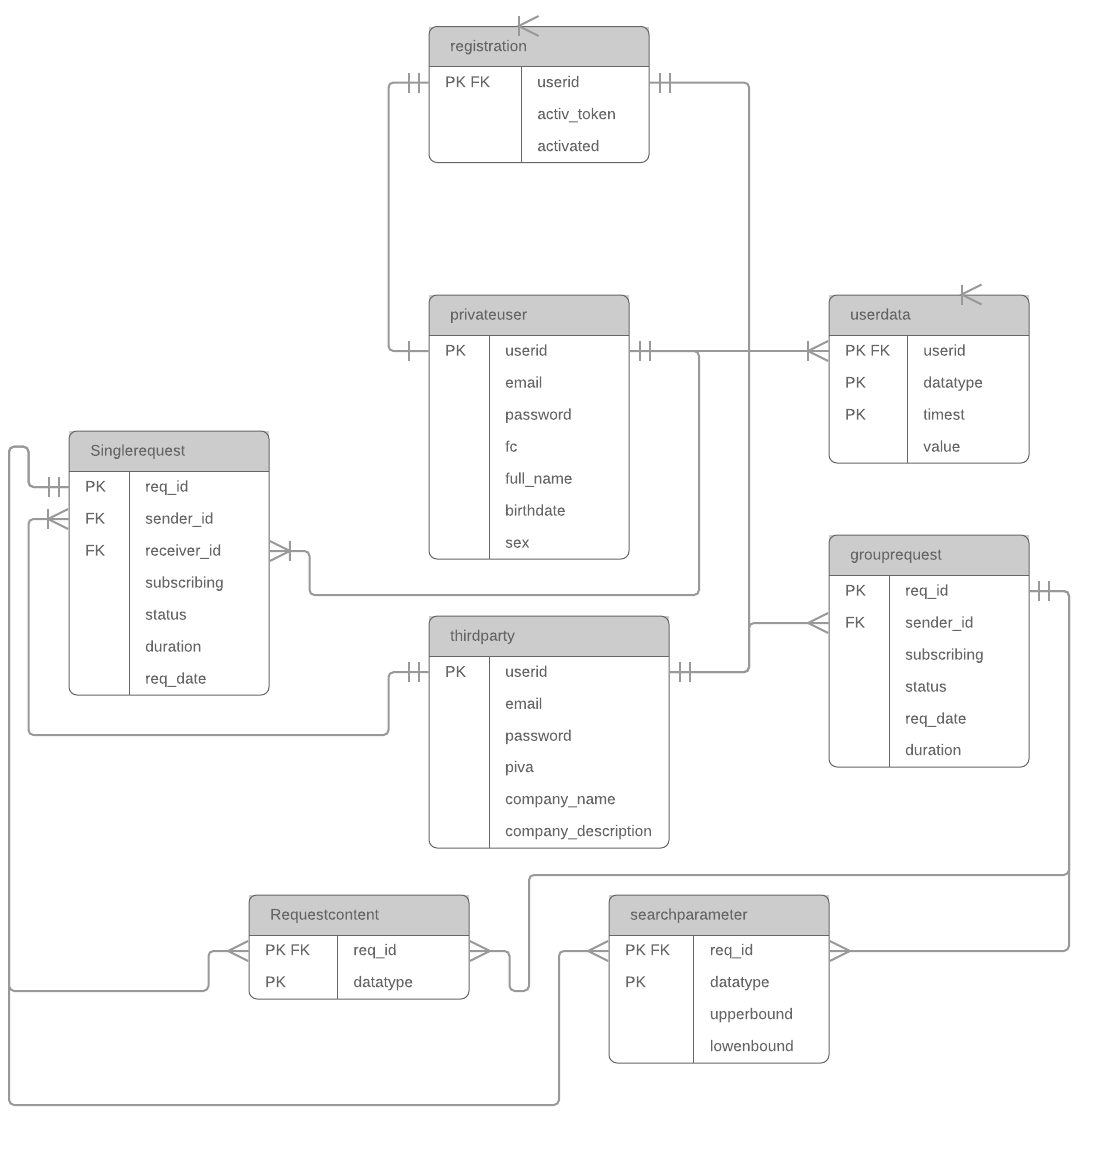
\includegraphics[width=15cm]{DBModel.png}
		\caption{Database ER diagram}
		\label{fig:COMPDIA}
	\end{figure}
	
	
	\subsubsection{Enums}
	Some custom data types have been defined to support the storage of health data and other various information such as the gender of the {\it Private User} and the status of a {\it Single Request}. The table down below shows the detail of each of them.
	\begin{longtable}{| p{2 cm} | p{7 cm} |} \hline
		ENUM & VALUES \\ \hline
		datatype & standinghours, heartrate, distancewalkingrunning, sleepinghours, weight, height, age, activeenergyburned, stepcount, systolic\_pressure, diastolic\_pressure \\ \hline
		gender & F, M \\ \hline
		requeststatus & pending, accepted, refused\\ \hline
		\caption{Enums}	
	\end{longtable}
	
	\subsubsection{Tables description}
	Here follows an accurate description of how all the tables designed in the previous document (See Design Document) have been implemented. The description includes for each table the column name, the data type, if it is a primary key and if it is nullable.
	\newline
	\newline
	\indent{\bf Group Request} 
	\renewcommand*{\arraystretch}{1.4}
	\begin{longtable}{| p{3 cm} | p{2 cm} | p{2 cm} | p{2 cm} |} \hline
		Column name & Data type & PK & Nullable \\ \hline
		duration & integer & NO & YES \\ \hline
		req\_date & date & NO & NO \\ \hline
		req\_id & integer & YES & NO \\ \hline
		sender\_id & varchar & NO & NO \\ \hline
		status & requeststatus & NO & NO \\ \hline
		subscribing & boolean & NO & NO \\ \hline
	\end{longtable}
	
	\vspace{\baselineskip}
	\vspace{\baselineskip}
	
	{\bf Singlerequest table} 
	\renewcommand*{\arraystretch}{1.4}
	\begin{longtable}{| p{3 cm} | p{2 cm} | p{2 cm} | p{2 cm} |} \hline
		Column name & Data type & PK & Nullable \\ \hline
		req\_id & integer & YES & NO \\ \hline
		sender\_id & varchar(10) & NO & NO \\ \hline
		receiver\_id & varchar(10) & NO & NO \\ \hline
		subscribing & boolean & NO & NO \\ \hline
		status & requeststatus & NO & NO \\ \hline
		duration & integer & NO & YES \\ \hline
		req\_date & date & NO & NO \\ \hline
	\end{longtable}
	
	\vspace{\baselineskip}
	\vspace{\baselineskip}
	
	{\bf Privateuser table} 
	\renewcommand*{\arraystretch}{1.4}
	\begin{longtable}{| p{3 cm} | p{2 cm} | p{2 cm} | p{2 cm} |} \hline
		Column name & Data type & PK & Nullable \\ \hline
		userid & varchar(10) & YES & NO \\ \hline
		email & varchar(40) & NO & NO \\ \hline
		password & varchar(100) & NO & NO \\ \hline
		fc & char(16) & NO & NO \\ \hline
		full\_name & varchar(30) & NO & YES \\ \hline
		birthdate & date & NO & YES \\ \hline
		sex & gender & NO & NO \\ \hline
	\end{longtable}
	
	\vspace{\baselineskip}
	\vspace{\baselineskip}
	
	{\bf Thirdparty table table} 
	\renewcommand*{\arraystretch}{1.4}
	\begin{longtable}{| p{3 cm} | p{2 cm} | p{2 cm} | p{2 cm} |} \hline
		Column name & Data type & PK & Nullable \\ \hline
		userid & varchar(10) & YES & NO \\ \hline
		email & varchar(40) & NO & NO \\ \hline
		password & varchar(100) & NO & NO \\ \hline
		piva & char(11) & NO & NO \\ \hline
		company\_name & varchar(20) & NO & YES \\ \hline
		company\_description & varchar(100) & NO & YES \\ \hline
	\end{longtable}
	
	\vspace{\baselineskip}
	\vspace{\baselineskip}
	
	{\bf Registration table} 
	\renewcommand*{\arraystretch}{1.4}
	\begin{longtable}{| p{3 cm} | p{2 cm} | p{2 cm} | p{2 cm} |} \hline
		Column name & Data type & PK & Nullable \\ \hline
		activ\_token & varchar(11) & YES & NO \\ \hline
		activated & boolean & NO & NO \\ \hline
		userid & varchar(10) & YES & NO \\ \hline
	\end{longtable}
	
	\vspace{\baselineskip}
	\vspace{\baselineskip}
	
	{\bf Requestcontent table} 
	\renewcommand*{\arraystretch}{1.4}
	\begin{longtable}{| p{3 cm} | p{2 cm} | p{2 cm} | p{2 cm} |} \hline
		Column name & Data type & PK & Nullable \\ \hline
		req\_id & integer & YES & NO \\ \hline
		datatype & datatype & YES & NO \\ \hline
	\end{longtable}
	
	\vspace{\baselineskip}
	\vspace{\baselineskip}
	
	{\bf Searchparameter table} 
	\renewcommand*{\arraystretch}{1.4}
	\begin{longtable}{| p{3 cm} | p{2 cm} | p{2 cm} | p{2 cm} |} \hline
		Column name & Data type & PK & Nullable \\ \hline
		req\_id & integer & YES & NO \\ \hline
		datatype & datatype & YES & NO \\ \hline
		lowerbound & integer & NO & YES \\ \hline
		upperbound & integer & NO & YES \\ \hline
	\end{longtable}
	
	\vspace{\baselineskip}
	\vspace{\baselineskip}
	
	{\bf Userdata table} 
	\renewcommand*{\arraystretch}{1.4}
	\begin{longtable}{| p{3 cm} | p{2 cm} | p{2 cm} | p{2 cm} |} \hline
		Column name & Data type & PK & Nullable \\ \hline
		userid & varchar(10) & YES & NO \\ \hline
		datatype & datatype & YES & NO \\ \hline
		timest & timestamp & YES & NO \\ \hline
		value & float8 & NO & NO \\ \hline
	\end{longtable}
	
	\subsection{XCode project structure}
	In this section we will describe the structure of our client application. It is implemented as an iOS Application using Swift programming language. The structure of the Xcode Project follows Apple\textsc{\char13}s  best practice guidelines on the MVCS design pattern. As a result, all classes are organized in four sections: Views, Controllers, Model and Utilities. Controllers in Swift include also ViewControllers, classes merging features of both views and controllers such as being responsible for the handling and updating the content of views, responding to their interaction with the user and for coordinating with other objects such as other controllers in the app.
	In the following paragraphs we will details each section with its main classes and functionalities.
	
	\subsubsection{Views}
	In this section we will describe how all views are implemented and organized within the project. Every view has been designed starting from a Storyboard, a unique XCode file that allows to prototype and design multiple views and connect them with each other. The project contains a total of three storyboards: “SingleUser.storyboard”, “ThirdParty.storyboard” and “Main.storyboard”, each containing a sequence of views belonging to a same section. Every view in the storyboards is connected to a specific subclass of UIViewController responsible for its content and its interaction with all other objects. \newline
	\newline
	The {\bf “Main.storyboard”} represents the sequence of views that are displayed when a user has not logged into his account. The user may either create a new {\it Single User} or {\it Third Party} account or log in with his credentials. When a user successfully enters his credentials a {\it segue} is wired programmatically to connect the current view controller to the following one to be visualized. For this purpose, the Main.storyboard keeps a reference to both “SingleUser.storyboard” and “ThirdParty.storyboard”. \newline
	\newline
	The  {\bf “SingleUser.storyboard”} contains all views that can be accessed by a user when he has logged into a {\it Single User} account. There are three main views connected to each other by a tab bar controller. Each view is associated to a tab: MyHealth, MyFollowers and MySettings. The first view is responsible for the health monitoring feature. It displays simple bar and bubble charts to get immediate information regarding the user\textsc{\char13}s health status and the comparison with the average for his age. MyFollowers is organized with a table view with custom cells to display all requests directed to that user. All the contained requests are either past ones or pending ones to be accepted or refused. A navigation bar is also used to retrieve a specific one. Finally, the MySettings view contains all general information associated to the user\textsc{\char13}s account, such as email, password and birth date, and enables their editing.\newline
	\newline
	The {\bf “ThirdParty.storyboard”} contains all views that can be accessed by a {\it Third Party} user when he logs into his account. As for the previous storyboard, all views are organized by a tab bar controller. Each view is associated to one of the three tabs: Research, History and Settings. With the Research view a {\it Third Party} user can create either a single or group request by selecting its filters onto the display. The History tab allows to retrieve all past and current requests and check whether they are still pending or have been accepted or refused. Finally the Settings sections displays all the general information associated to the {\it Third Party} account and enables their editing.\newline
	\newline
	\noindent
	{\bf Cells} \newline
	Under this folder are stored all the classes used to represent and manage a custom cell in a UITableViewController.
	\begin{itemize}
		\item {\bf SURequestCell.swift}: is the cell used in {\it {\it Single User}}\textsc{\char13}s MyFollower tab table view. Its content shows information about a {\it Single Request} sent to the logged {\it {\it Single User}}. Namely it shows the {\it {\it Third Party}} name, the requested datatypes and the application of a subscription. In case of a pending request two buttons are also added in order to either accept or refuse it.
		\item {\bf TPRequestCell.swift}: this cell represents the content of a {\it Single Request} in the MyHistory tab of a {\it {\it Third Party}}. It shows the name of the {\it {\it Single User}} the request was sent to, the requested datatypes, the date and whether it is subscribing or not. The cell also present a toggle that allow a {\it {\it Third Party}} to end a subscribing request before its expiring date. Finally there is a download button that allow the user to download the csv containing the data of an accepted request.
		\item {\bf TPGroupRequestCell.swift}: this cell is used in the same context of the previous one but to represent the content of {\it Group Requests}. The main difference lies in the cell layout.
	\end{itemize}
	
	\subsubsection{Controllers}
	{\bf Main Controllers}
	\begin{itemize}
		\item {\bf LoginViewController.swift}: this is the initial view controller and it handles login operations. Depending on the user interaction it can perform a segue to the Registration Controllers or, after sending a login request, perform a segue to {\it Single User} or {\it Third Party} storyboard. If the input credentials are invalid, an error prompt informs the user.
		
		\begin{figure}[H]%
			\centering
			\subfloat[Login view ]{{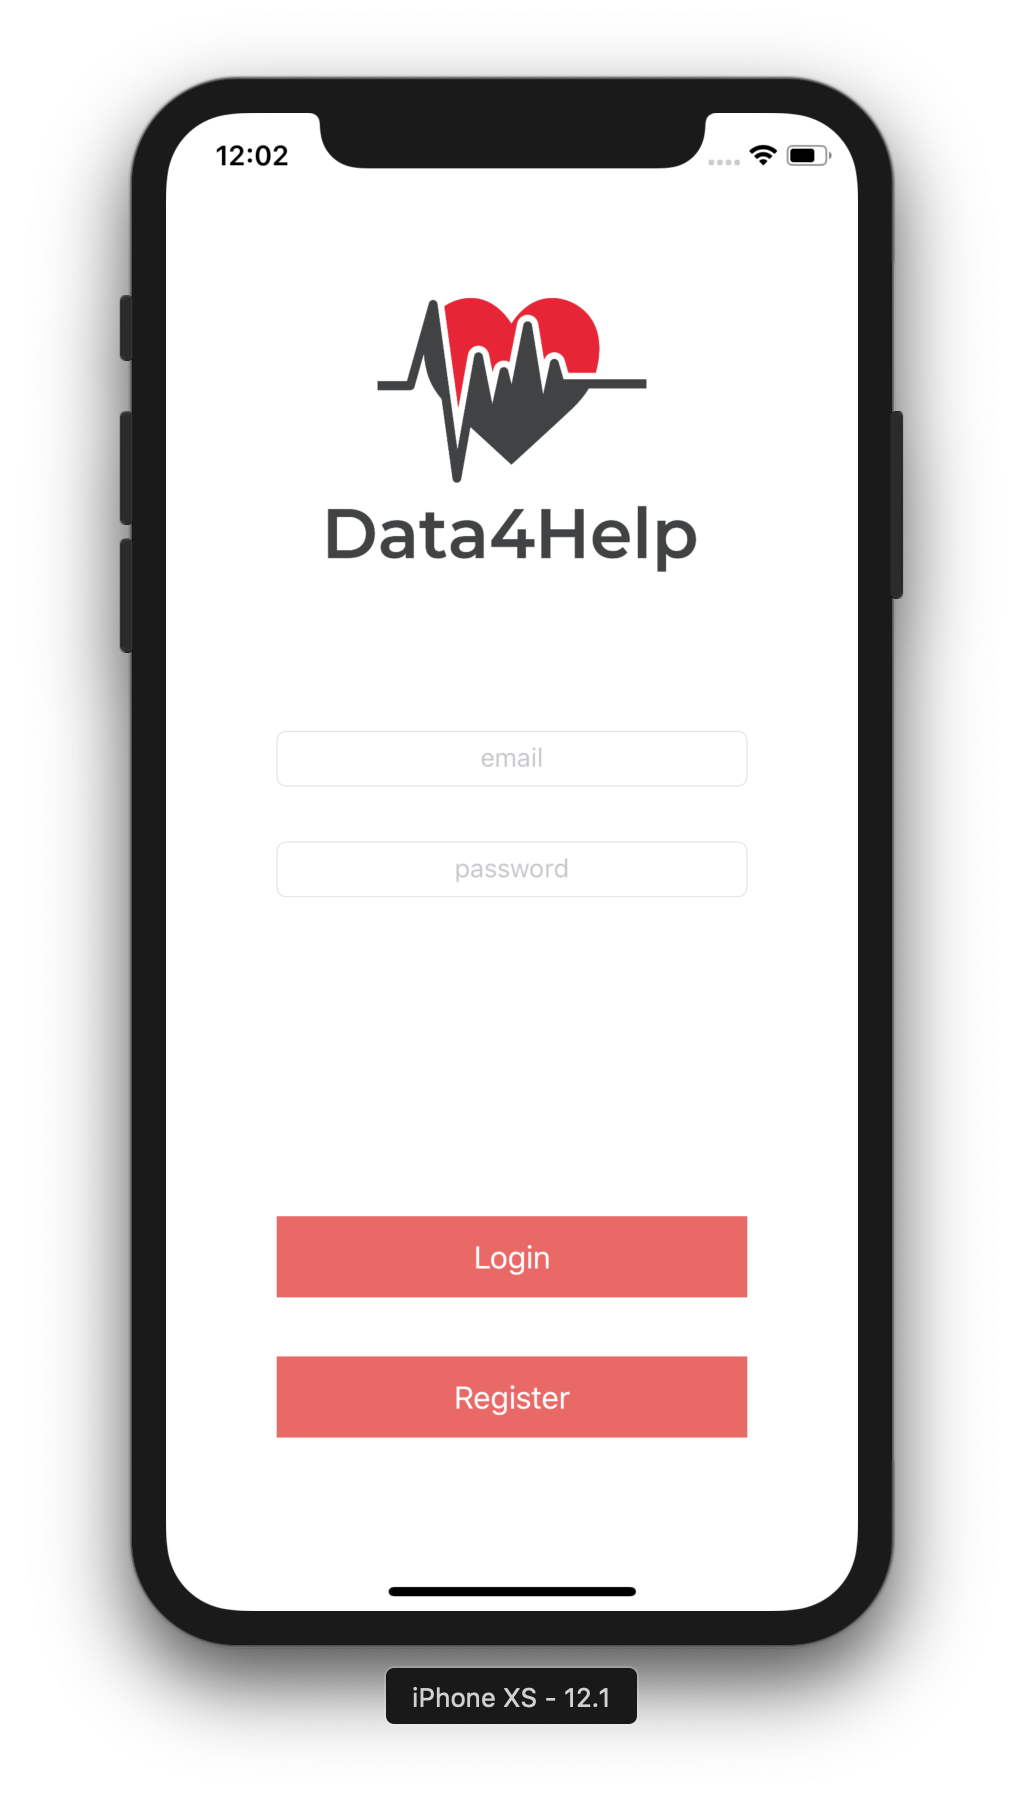
\includegraphics[width=5cm]{images/SimulatorScreenshots/login.png}}}%
			\qquad
			\subfloat[Login error ]{{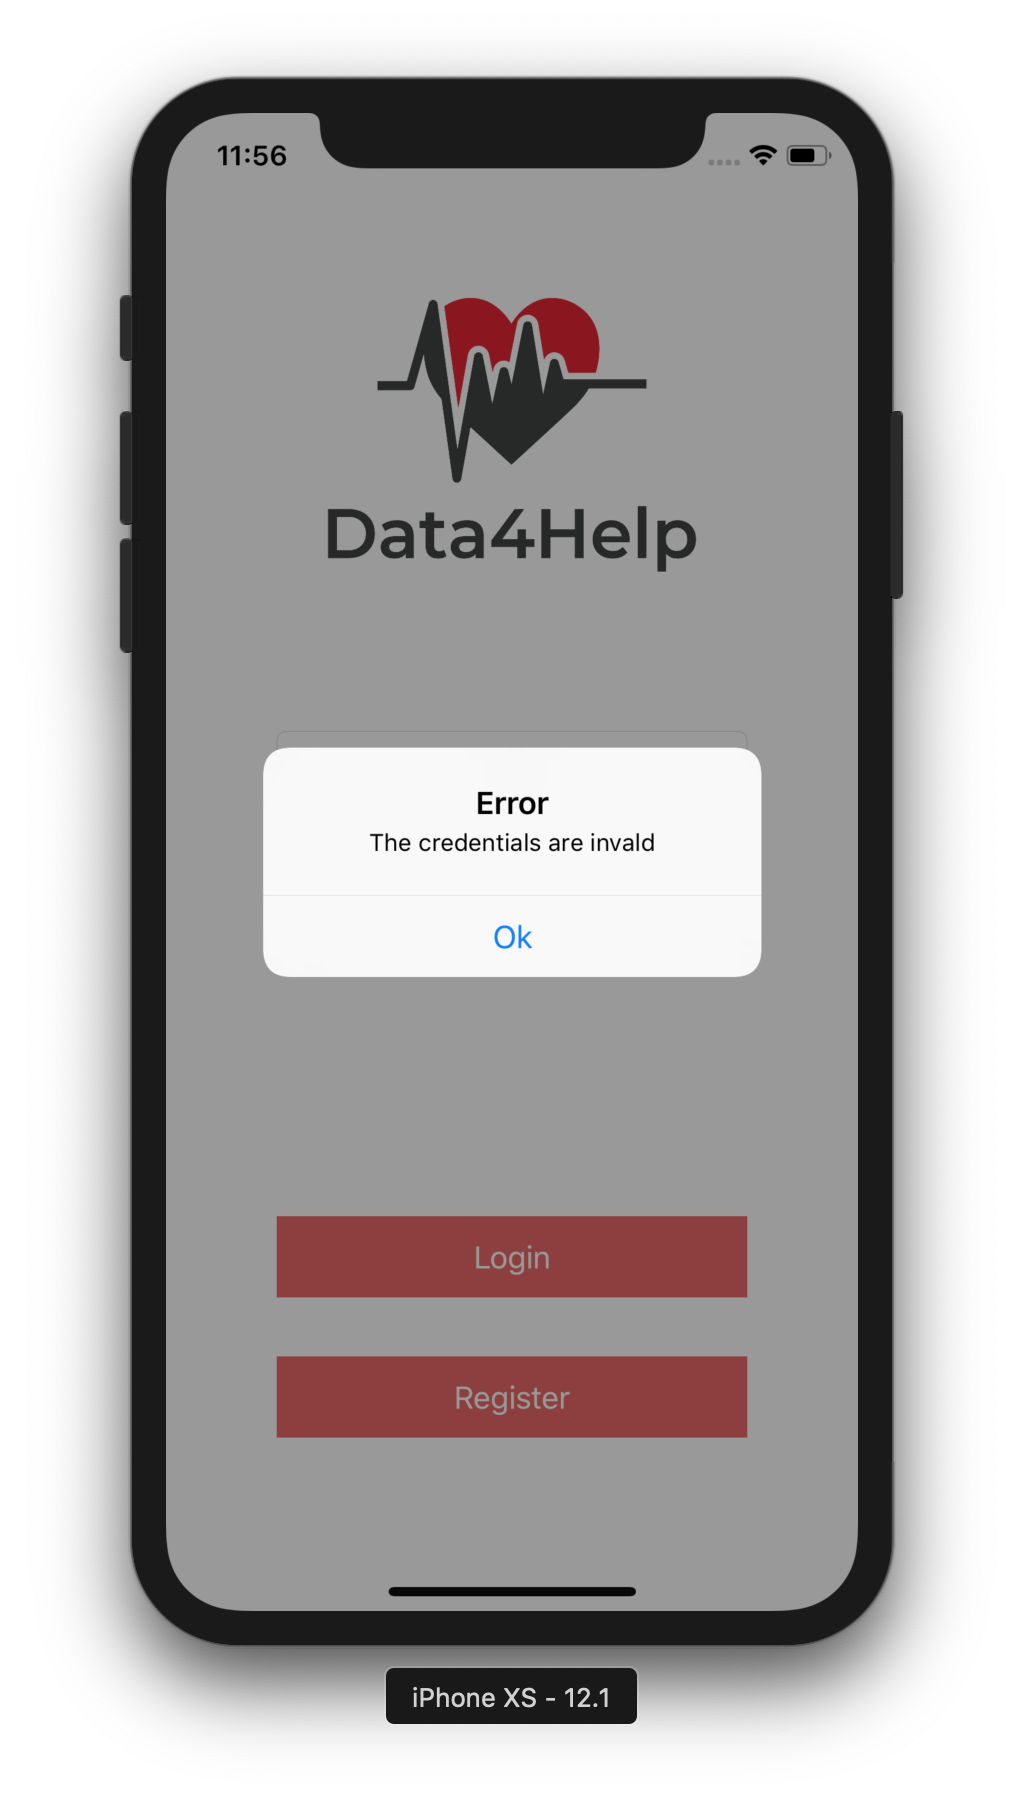
\includegraphics[width=5cm]{images/SimulatorScreenshots/error.png}} }%
			\caption{Login screenshots}%
			\label{fig:RequestTab}%
		\end{figure}
		
		\item {\bf SURegisterViewController.swift}: it shows the registration form for {\it Single Users} and sends registration requests to the backend. In case of successful response it performs a segue to login view.
		\item {\bf TPRegisterViewController.swift}: it shows the registration form for {\it Third Parties} and sends registration requests to the backend. In case of successful response it performs a segue to login view.
		\begin{figure}[H]%
			\centering
			\subfloat[{\it Single User} register view ]{{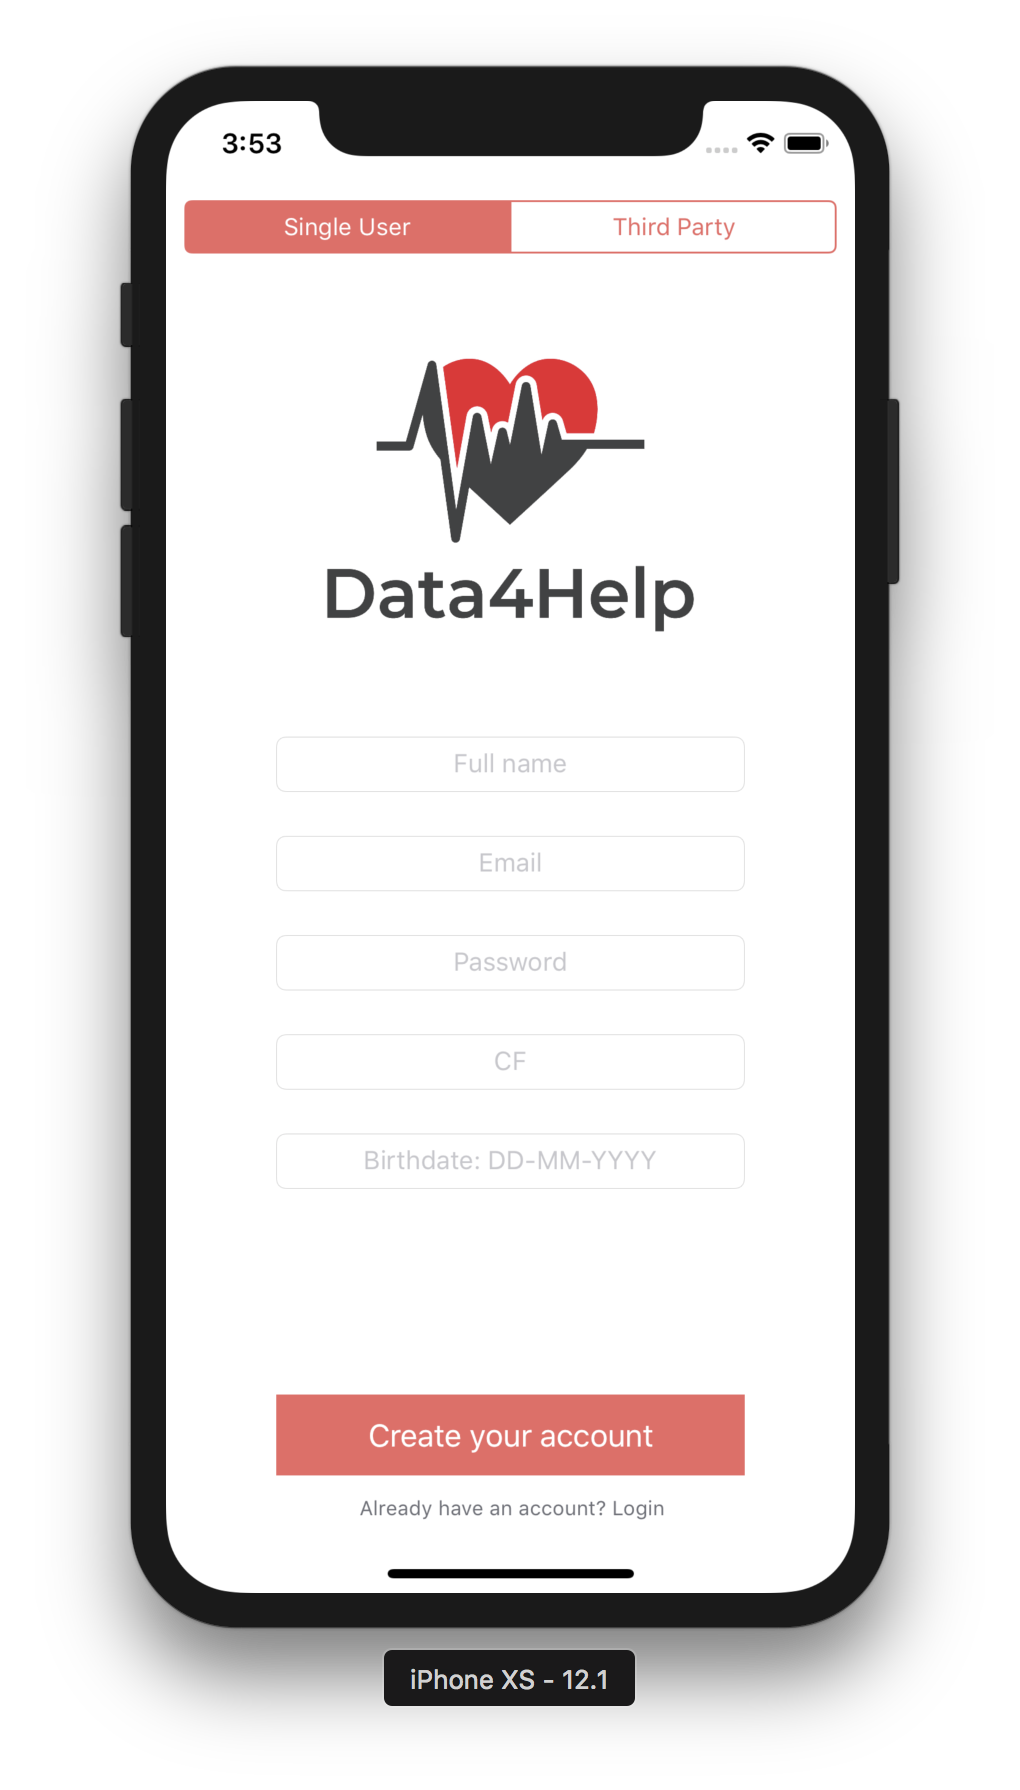
\includegraphics[width=5cm]{images/SimulatorScreenshots/suregister.png}}}%
			\qquad
			\subfloat[{\it Third Party} register view ]{{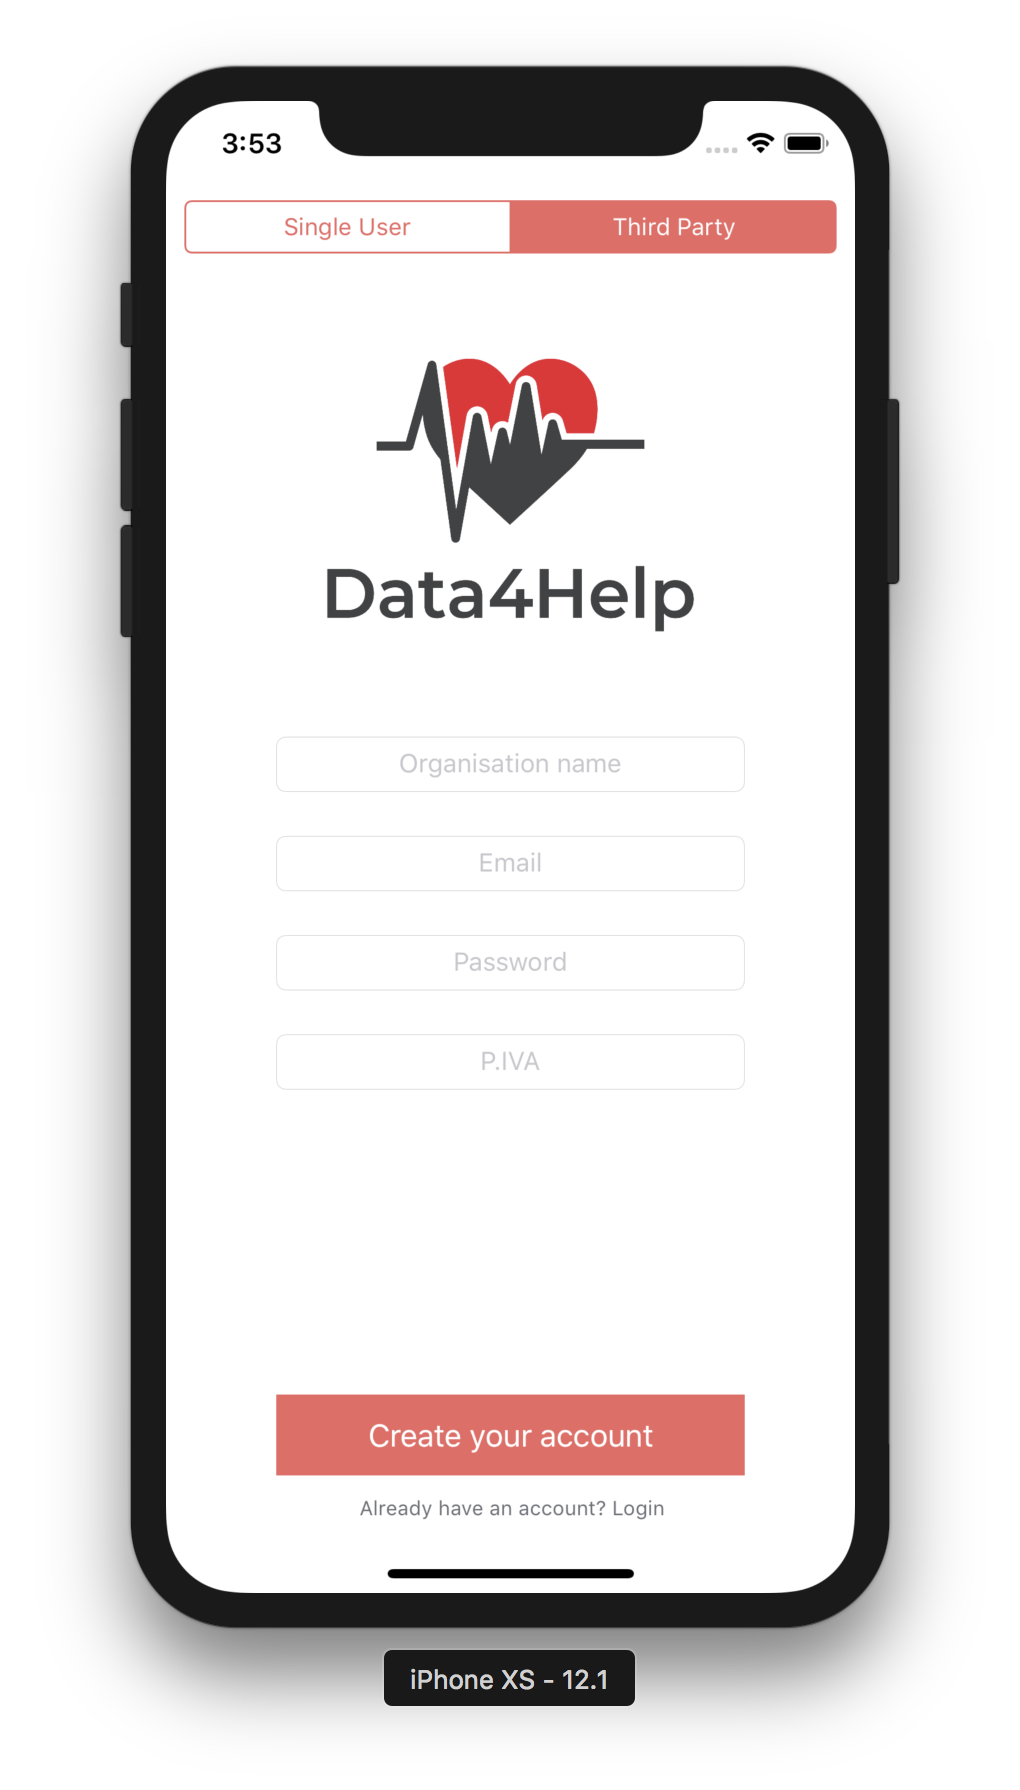
\includegraphics[width=5cm]{images/SimulatorScreenshots/tpregister.png}} }%
			\caption{Register views screenshots}%
			\label{fig:RequestTab}%
		\end{figure}
		\item {\bf TutorialViewController.swift}: it presents a list of simple instruction useful to decide what is the most suitable kind of profile for the new user. It also tells how to complete the account activation phase after signing up from the application.
		
		\begin{figure}[H]%
			\centering
			\subfloat[Tutorial page 1 ]{{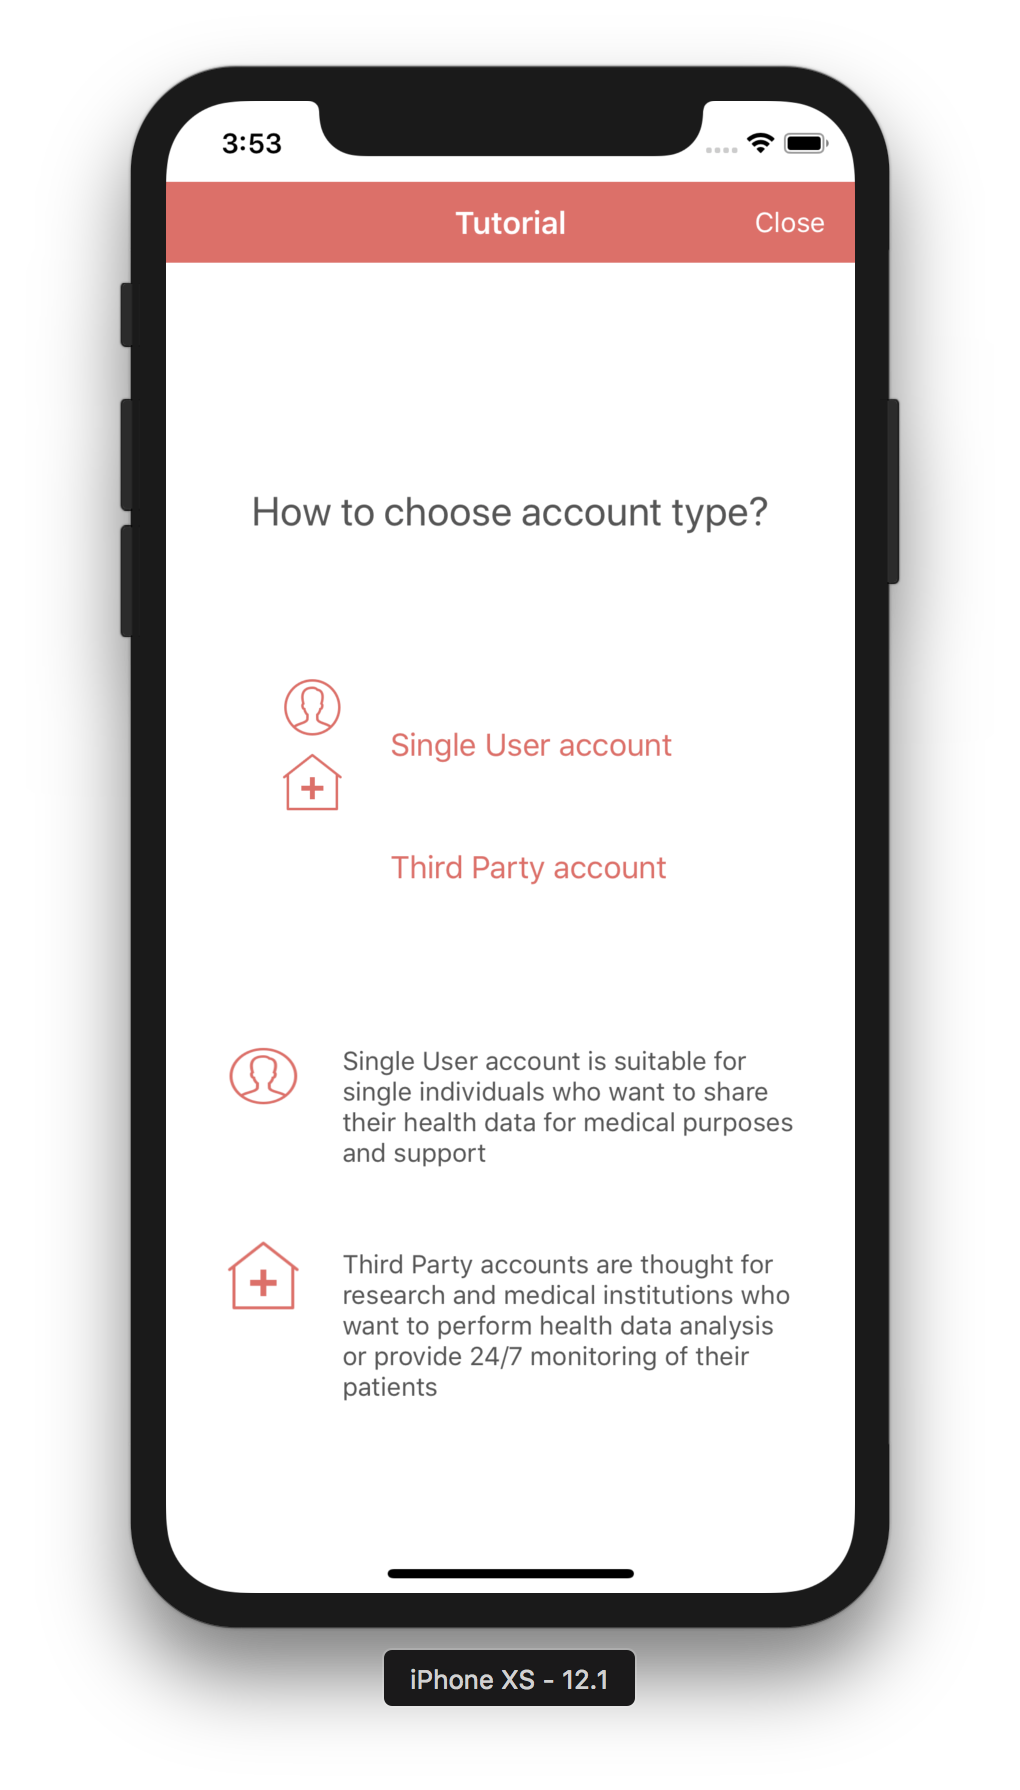
\includegraphics[width=5cm]{images/SimulatorScreenshots/tutorial1.png}}}%
			\qquad
			\subfloat[Tutorial page 2]{{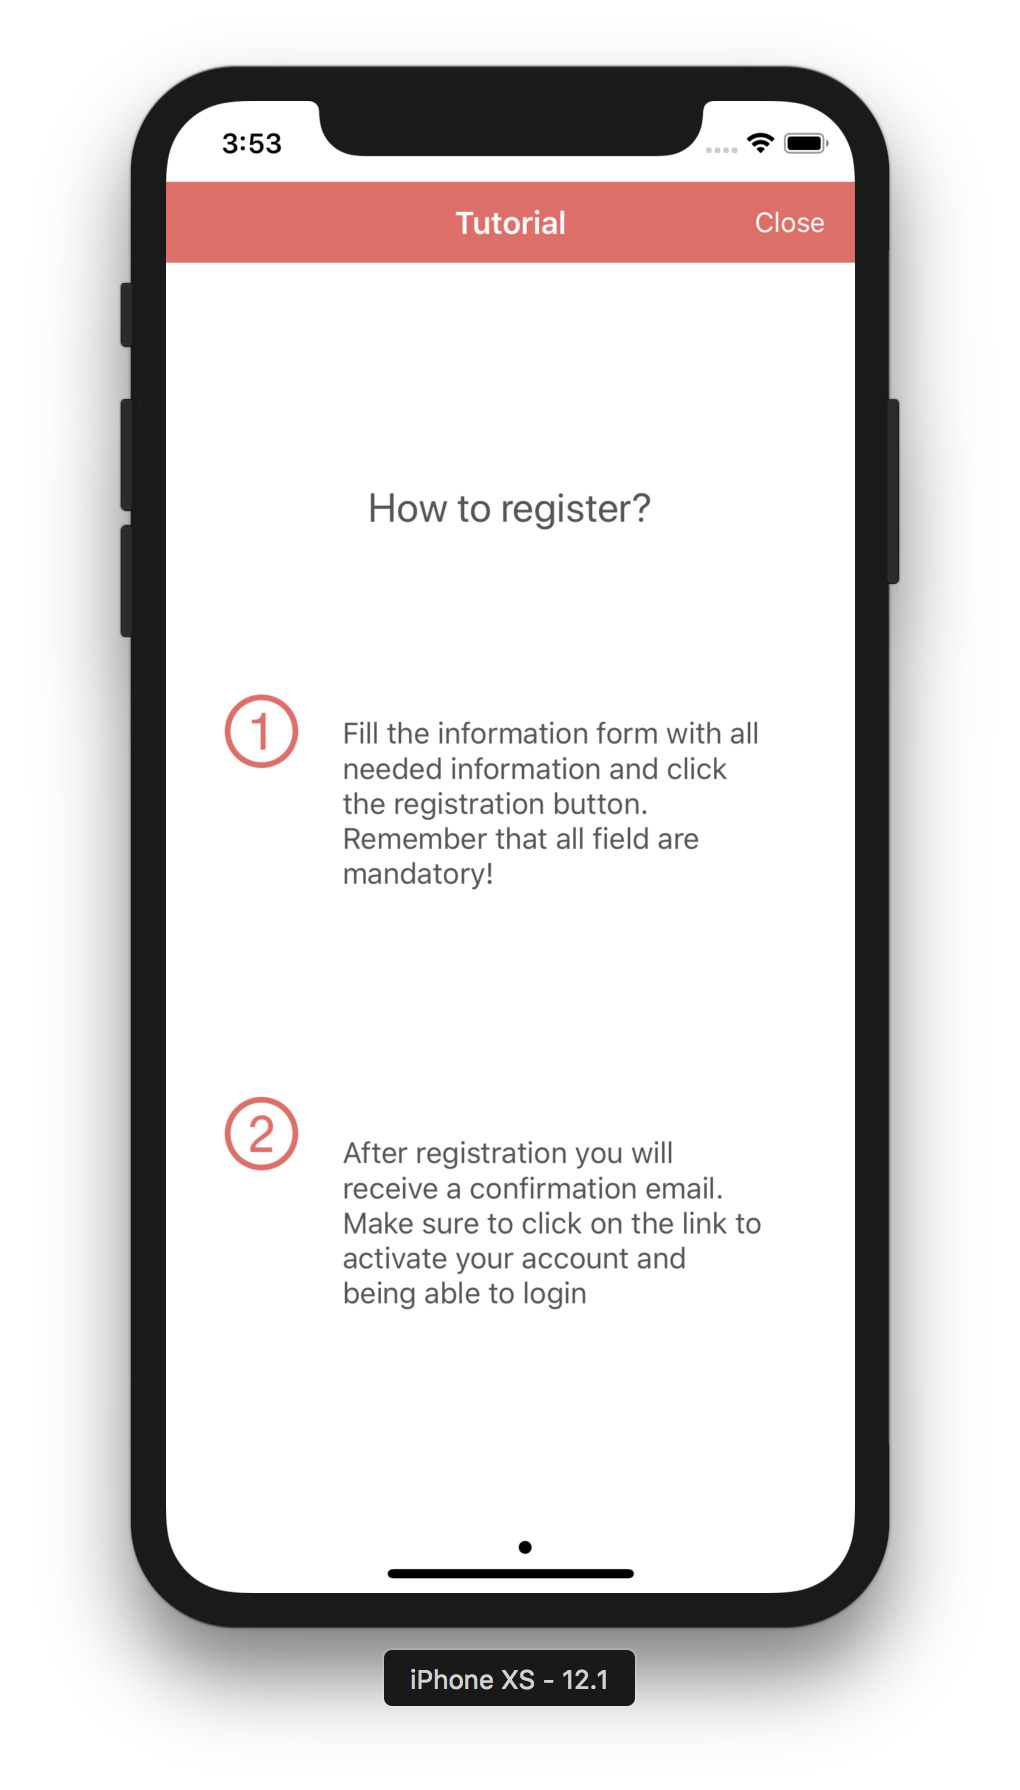
\includegraphics[width=5cm]{images/SimulatorScreenshots/tutorial2.png}} }%
			\caption{Tutorial view screenshots}%
			\label{fig:RequestTab}%
		\end{figure}
	\end{itemize}
	\vspace{\baselineskip}
	\noindent
	{\bf SU Controllers} \newline
	
	\indent{ 
		{\bf Settings controllers}
		\begin{itemize}
			\item {\bf SUSettings.swift}:  acts as a container for the views managed by SUViewSettings and SUEditSettings. These two views are alternatively shown to the user depending on whether he pressed an edit button in the top right corner of the screen. The view also present in the bottom part a button allowing to logout or to save the edited informations.
			\item {\bf SUViewSettings.swift}: manages the view containing the info and settings related to the logged {\it {\it Single User}}. They namely are full name, email, password (obscured), FC and birthdate.
			\item {\bf SUEditSettings.swift}: presents a layout almost identical to SUViewSettings but some field are presented as texfields in order to allow the editing of some information.
			
		\end{itemize}
		
		\begin{figure}[H]%
			\centering
			\subfloat[Settings view ]{{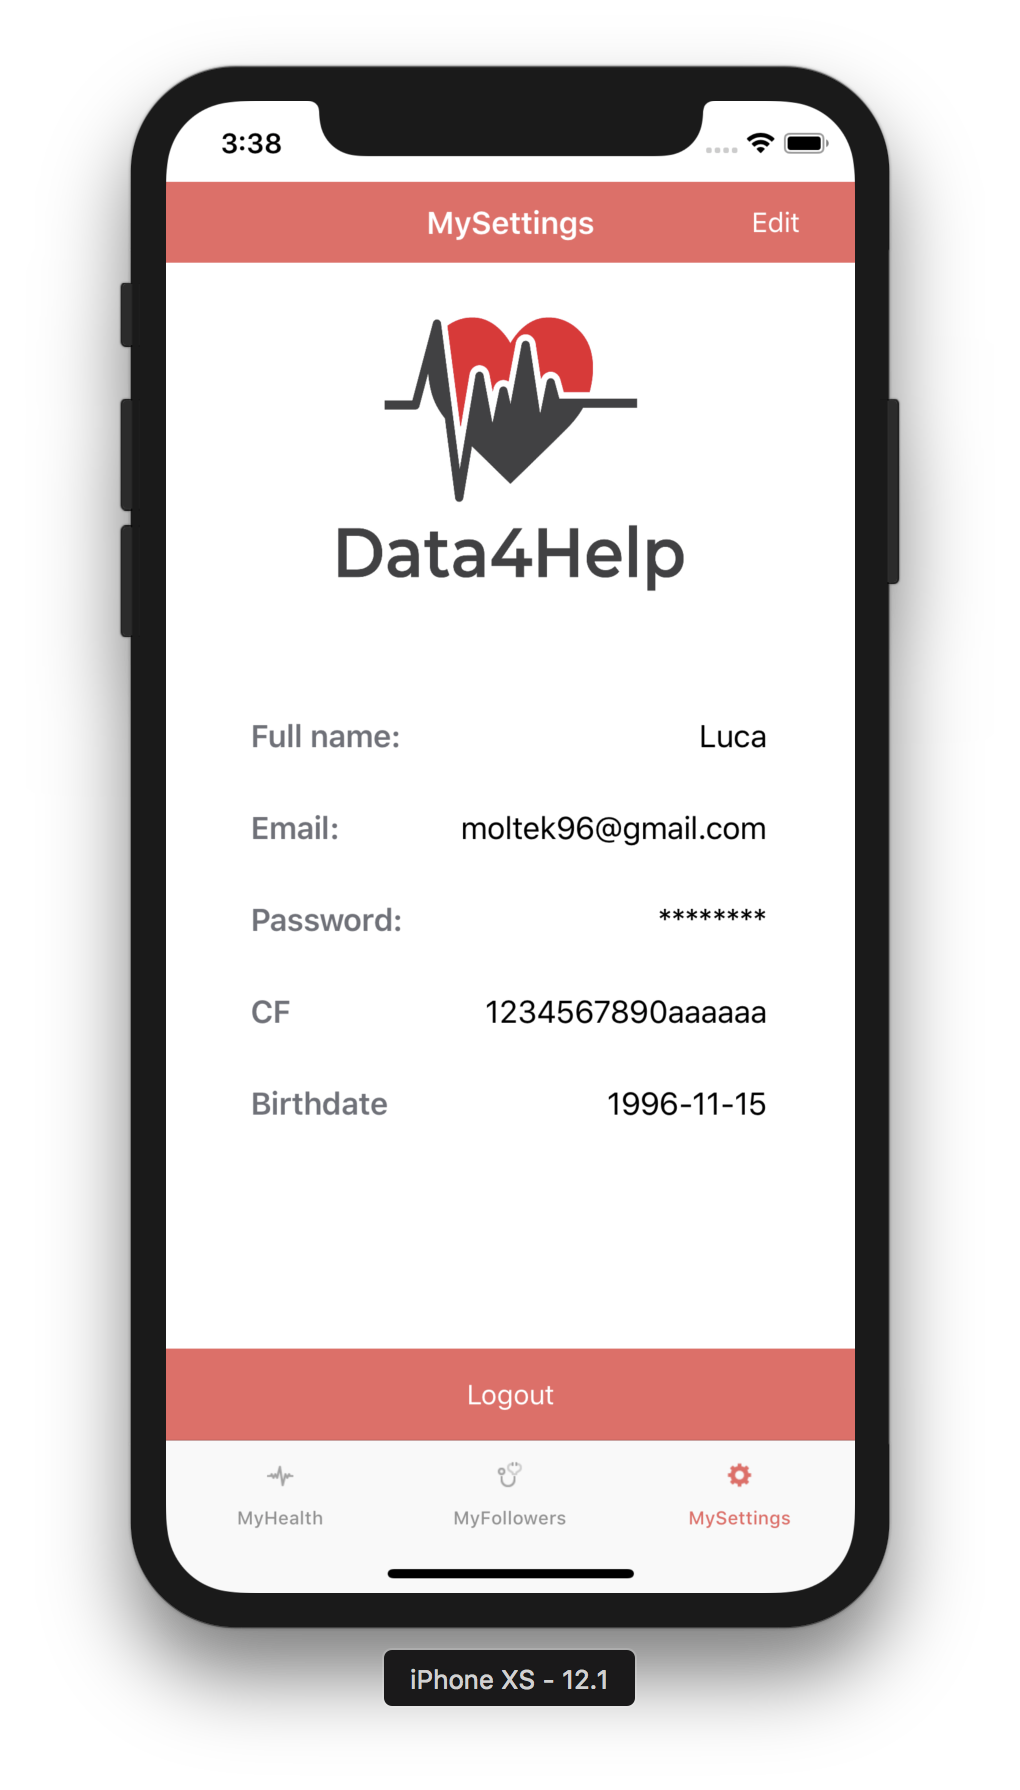
\includegraphics[width=5cm]{images/SimulatorScreenshots/susettings.png}}}%
			\qquad
			\subfloat[Edit settings]{{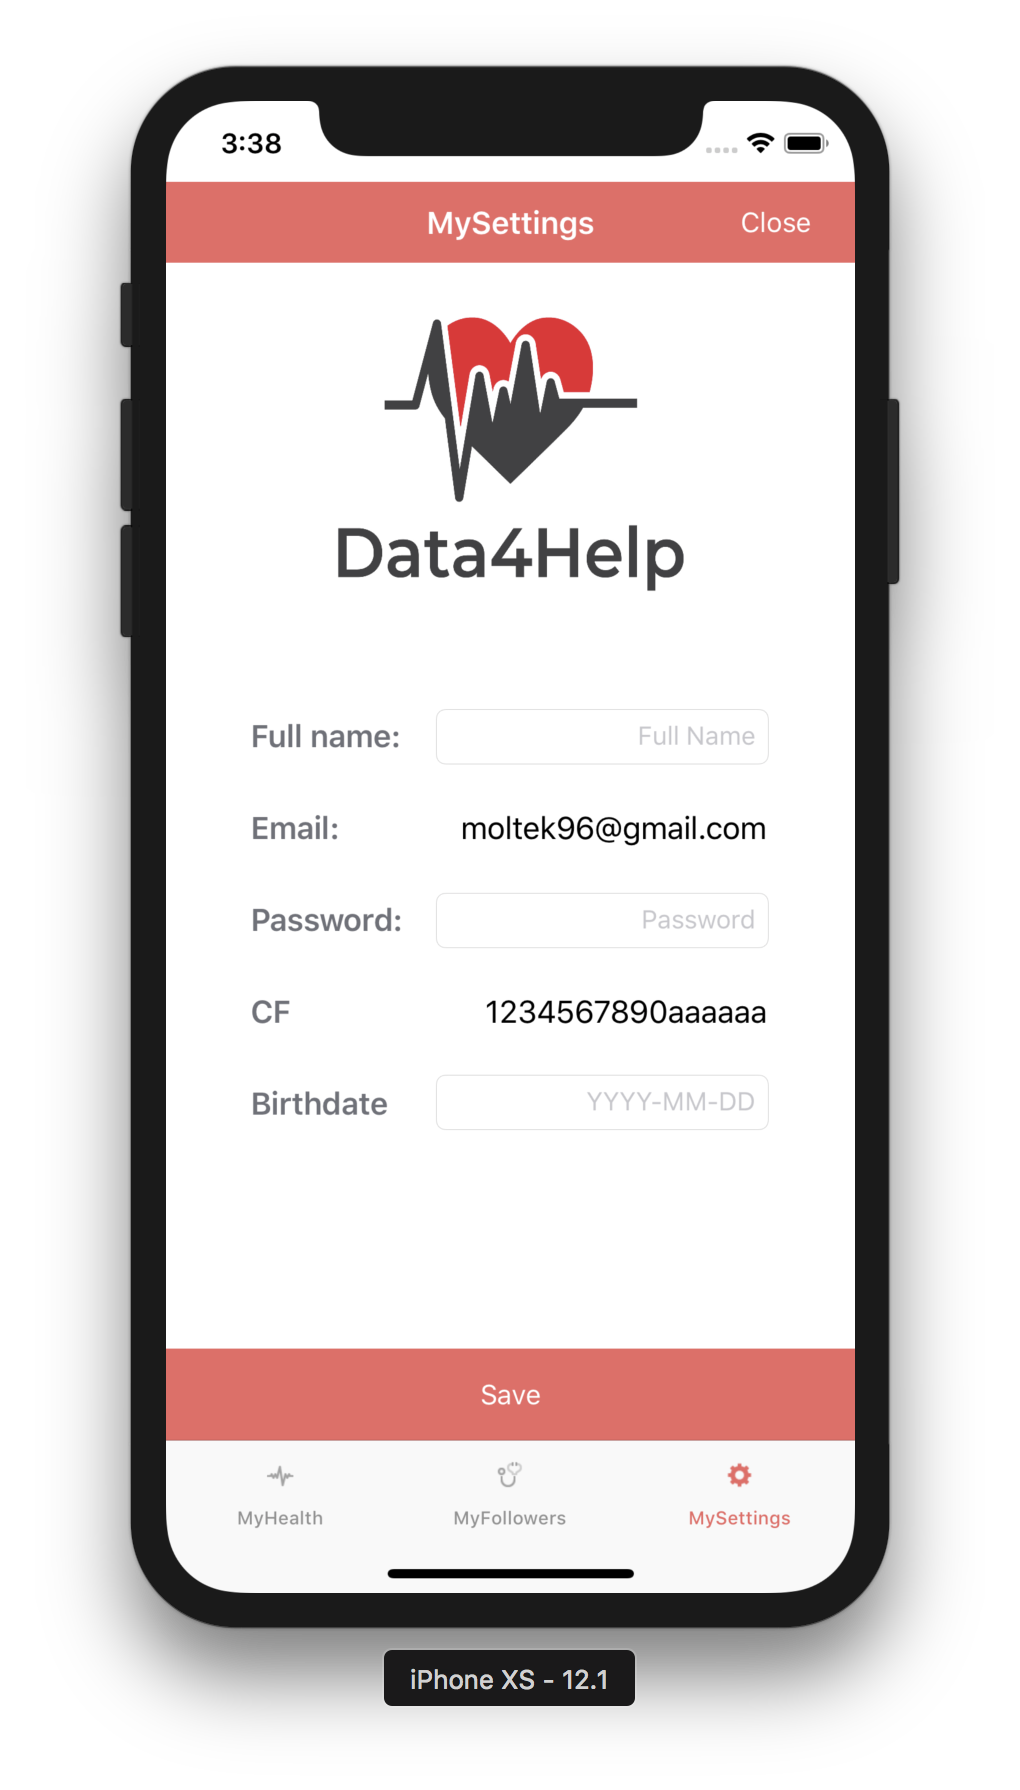
\includegraphics[width=5cm]{images/SimulatorScreenshots/sueditsettings.png}} }%
			\caption{{\it Single User} Settings tab screenshots}%
			\label{fig:RequestTab}%
		\end{figure}
		
		{\bf MyFollowers controllers}
		\begin{itemize}
			\item {\bf RequestController.swift}: it manages the UITableView containing all the received requests. The request are divided in three sections: accepted, pending and refused. It also provides a search bar to easily filter requests based on the sender name.
			\item {\bf MyCellDelegate.swift}: a protocol allowing SURequestCell class to call some methods from RequestController.
			
		\end{itemize}
		
		\begin{figure}[H]
			\center
			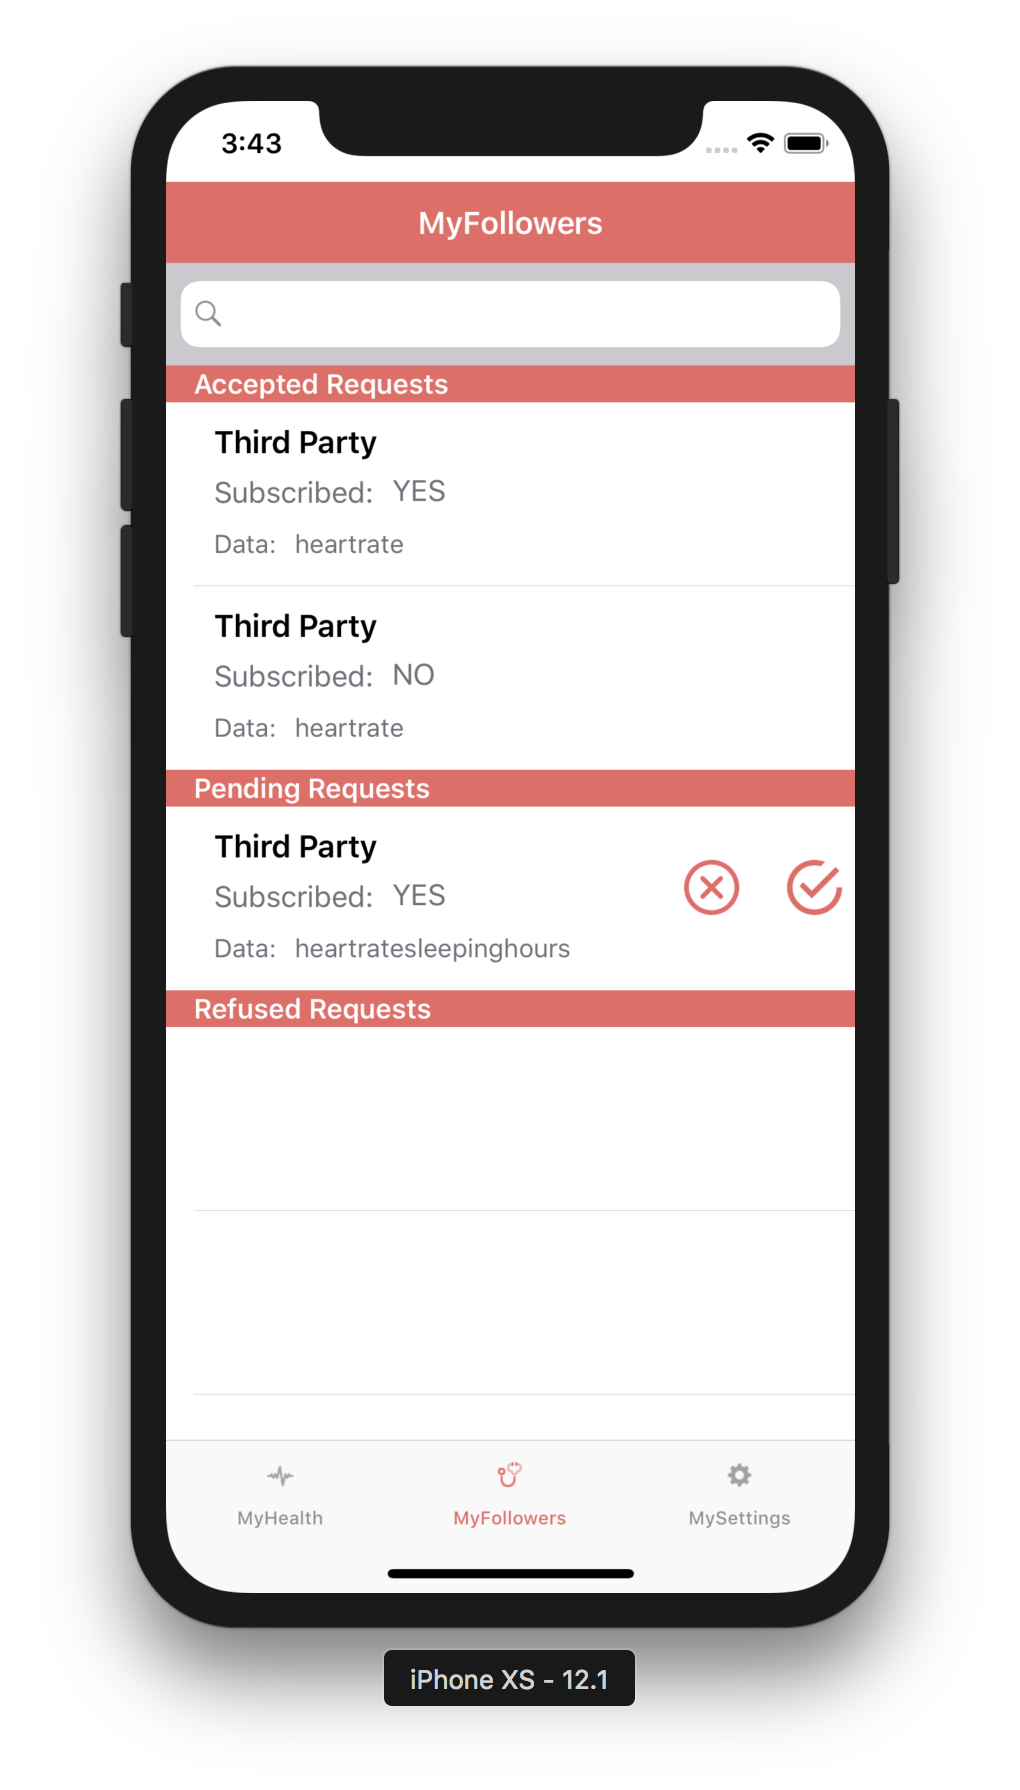
\includegraphics[width=5cm]{SimulatorScreenshots/myfollowers.png}
			\caption{MyFollower tab}
			\label{fig:Hist}
		\end{figure}
		
		{\bf MyHealth controllers}
		\begin{itemize}
			\item {\bf MyHealth.swift}: a subclass of UIViewController responsible for the behaviour of the MyHealth tab in the {\it {\it Single User}} interface. This class handles the user interaction with the {\it AutomatedSOS} button and with the bar and bubble charts displaying health data statistics inside the UIViewContiners. All charts are special UIView objects provided my the "Charts" framework. Their dataset can be refreshed by simply tapping onto them.
			\item {\bf AverageBarChartViewController}: a subclass of UIViewController responsible for setting up and reloading the data sets for a specific bar chart. This is the chart with two input data sets to compare: the average data values of the user and of all others of his age. All values are requested to the application server with a D4HStatisticsRequest.
			\item {\bf CurrentBarChartViewController}: a subclass of UIViewController responsible for setting up and reloading the data set of the bar chart containing the user\textsc{\char13}s current data. No request to the application server is required as all current values can be quickly retained by the local storage.
			\item {\bf BubbleChartViewController}: a subclass of UIViewController responsible for setting up and reloading the data set for the bubble chart. This charts shows for all types of data the minimum, average and maximum values of the current month.
			
		\end{itemize}
		
		\begin{figure}[H]%
			\centering
			\subfloat[Average bar chart ]{{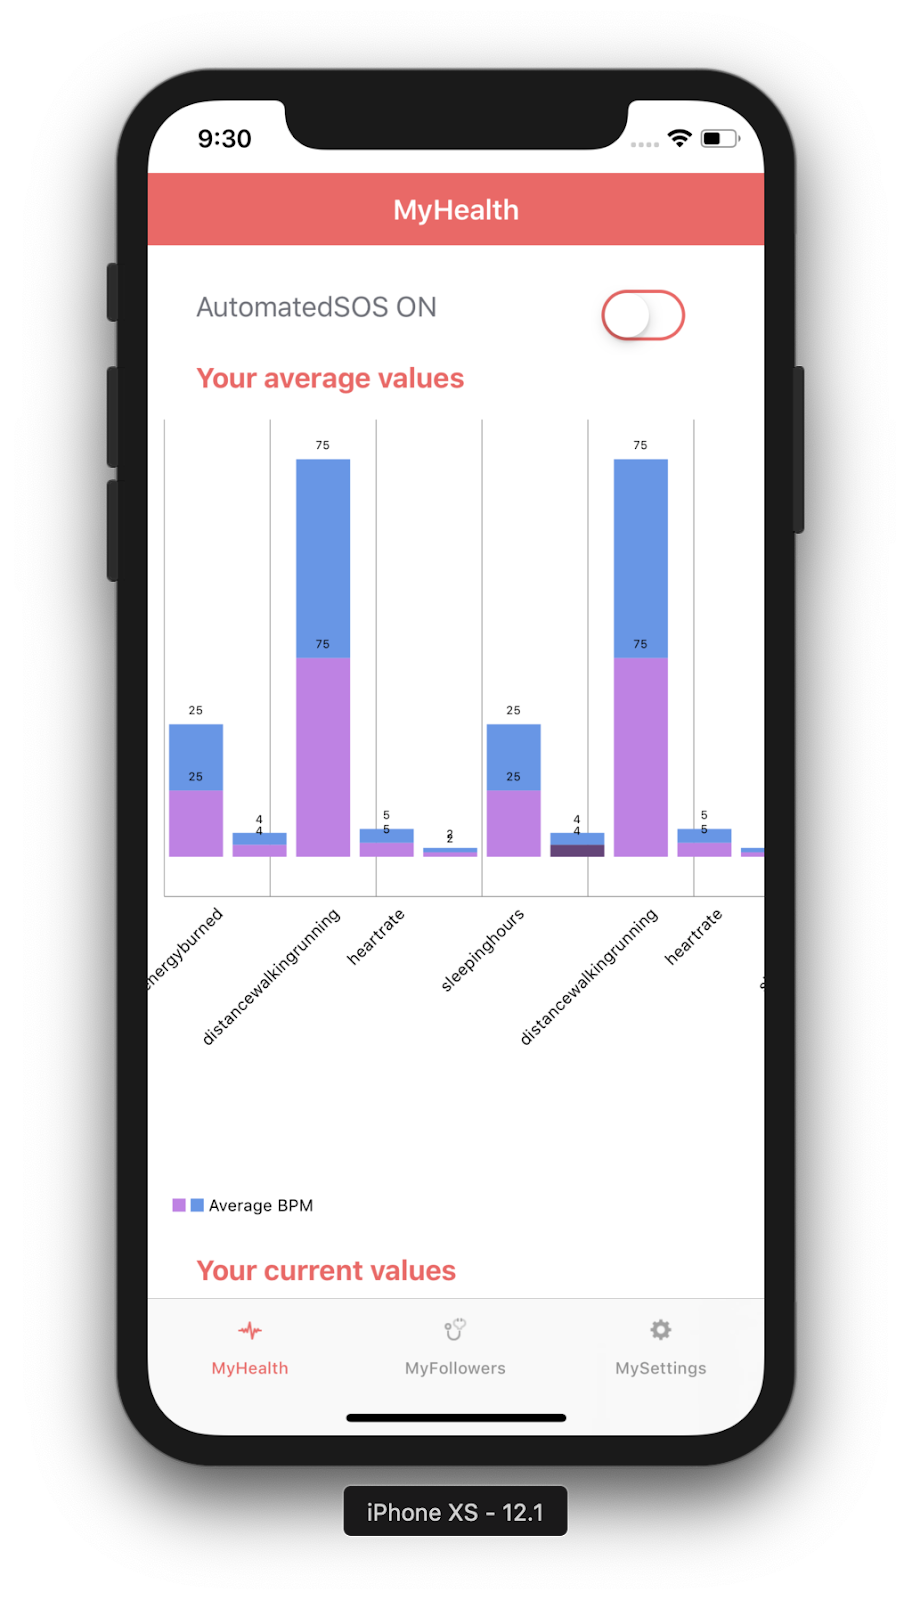
\includegraphics[width=5cm]{images/SimulatorScreenshots/myhealth1.png}}}%
			\qquad
			\subfloat[Current data bar chart ]{{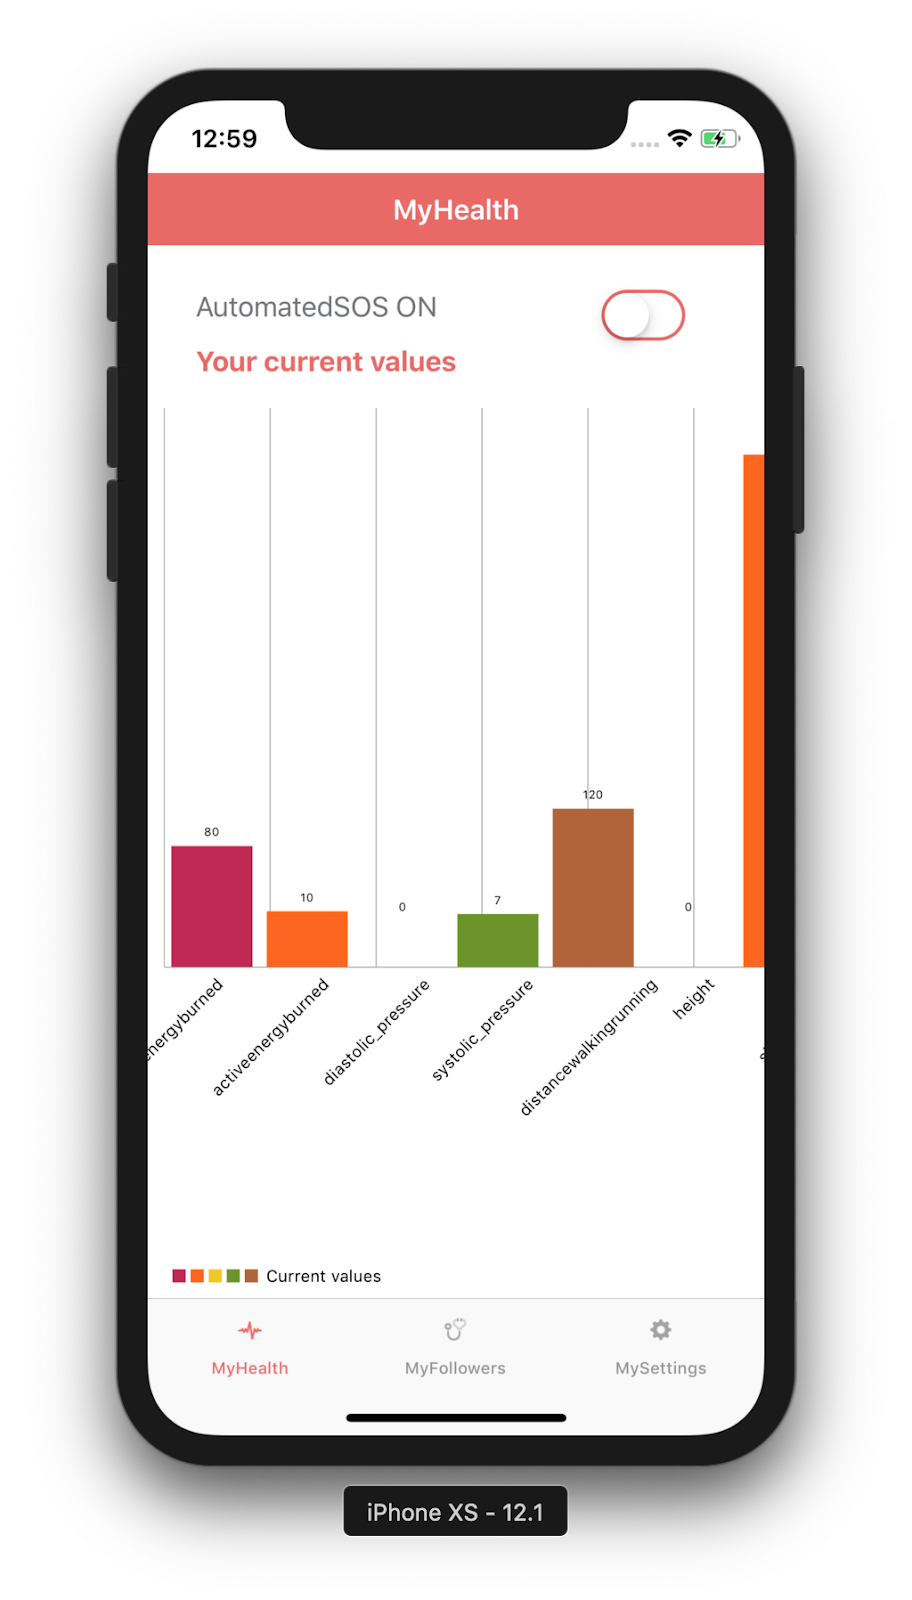
\includegraphics[width=5cm]{images/SimulatorScreenshots/myhealth2.png}} }%
			\qquad
			\subfloat[Bubble chart ]{{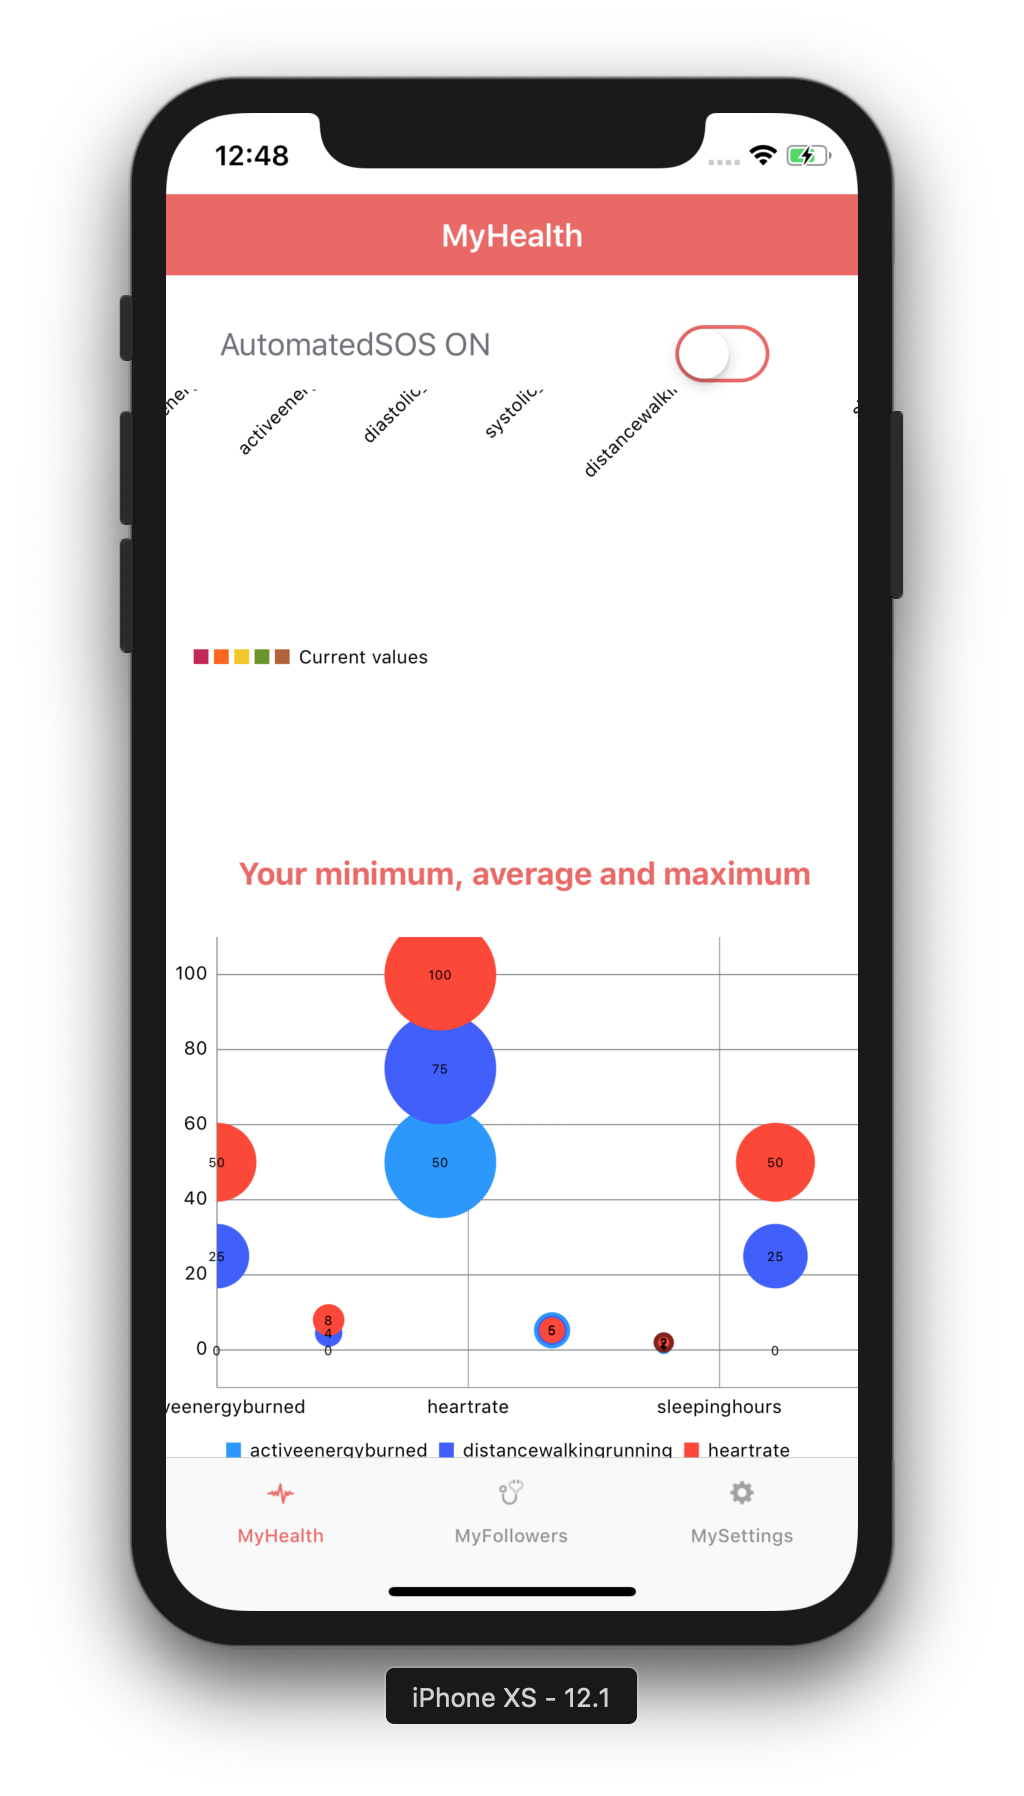
\includegraphics[width=5cm]{images/SimulatorScreenshots/myhealth3.png}} }%
			\caption{MyHealth tab screenshots}%
			\label{fig:RequestTab}%
		\end{figure}
		
	}
	\vspace{\baselineskip}
	\noindent
	{\bf TP Controllers} \newline
	
	\indent{ 
		{\bf Research controllers}
		\begin{itemize}
			\item {\bf SRequest.swift}: it manages the form used to define and perform a request to a {\it {\it Single User}}. Elements of this form are texfields to specify {\it {\it Single User}}\textsc{\char13}s FC or email and a sequence of toggles to specify the desired datatypes. At the bottom of the view a button allows to send the request to the backend.
			\item {\bf GRequest.swift}: it manages the form used to define and perform {\it Group Requests}. This form is made of two sections. The first presents a number of sliders and textfields used to define filtering parameters for the request. The second section contain a sequence of toggles used to specify the requested datatypes. At the bottom of the view a button allows to send the request to the backend.
			\item {\bf ResearchViewController.swift}: acts as a container for the views managed by SRequest and GRequest. These two views are alternatively shown to the user depending on whether he tapped one of the two sections of the segmented controller in the top part of the screen.
			
		\end{itemize}
		
		\begin{figure}[H]%
			\centering
			\subfloat[Group Request view ]{{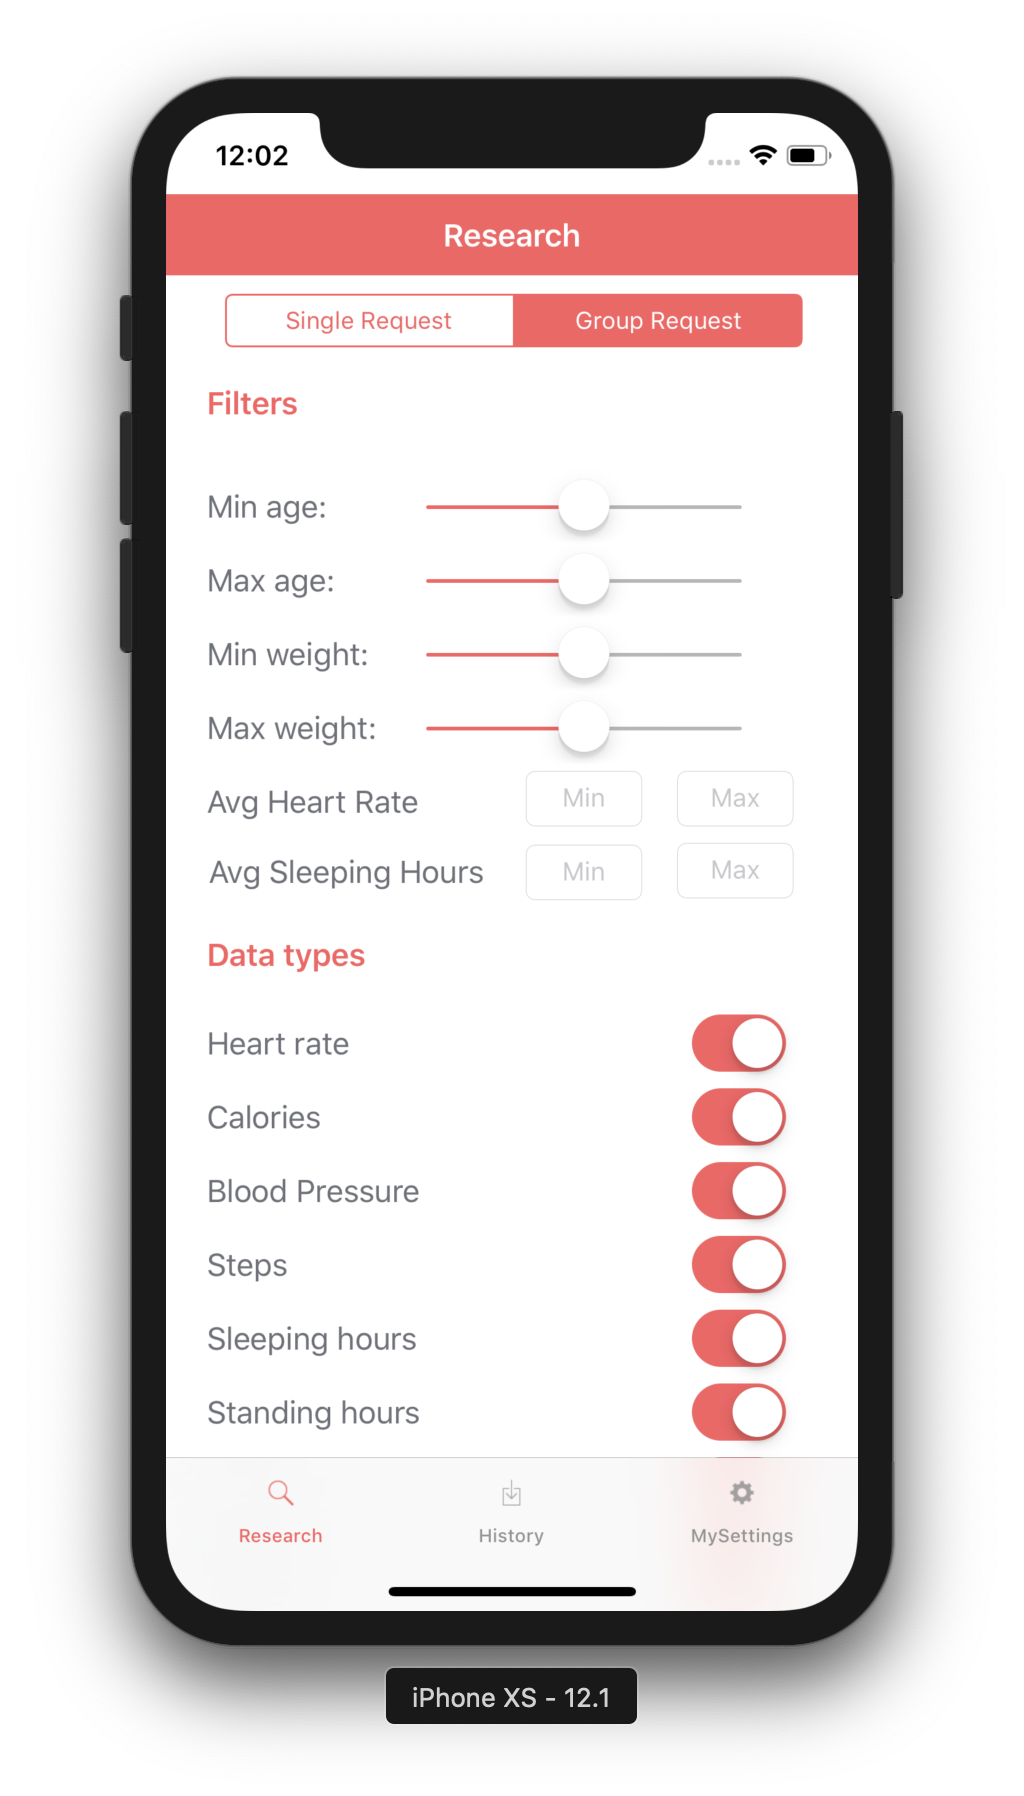
\includegraphics[width=5cm]{images/SimulatorScreenshots/grequests.png}}}%
			\qquad
			\subfloat[Single Request view ]{{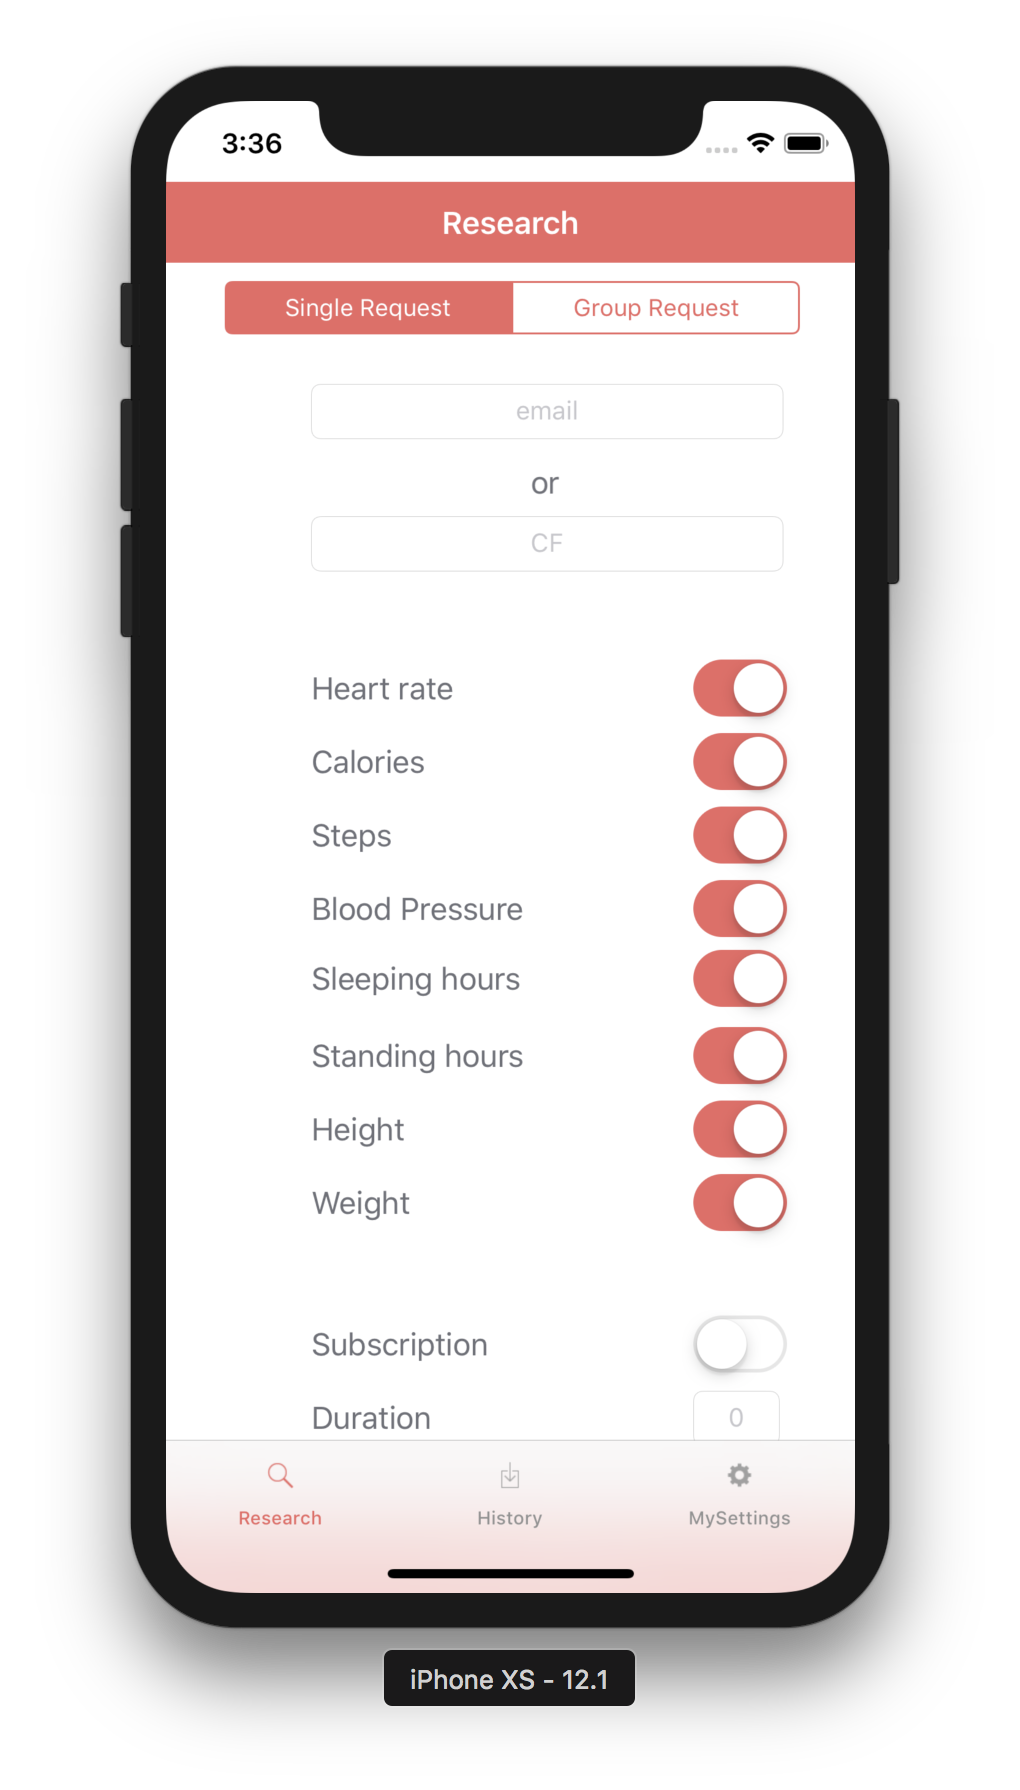
\includegraphics[width=5cm]{images/SimulatorScreenshots/singlerequest.png}} }%
			\caption{Research tab screenshots}%
			\label{fig:RequestTab}%
		\end{figure}
		
		{\bf Settings controllers}
		\begin{itemize}
			\item {\bf TPSettings.swift}:  acts as a container for the views managed by TPViewSettings and TPEditSettings. These two views are alternatively shown to the user depending on whether he pressed an edit button in the top right corner of the screen. The view also present in the bottom part a button allowing to logout or to save the edited informations.
			\item {\bf TPViewSettings.swift}: manage the view containing the info and settings related to the logged {\it Third Party}. They namely are full organisation name, email, password (obscured), PIVA and description.
			\item {\bf TPEditSettings.swift}: present a layout almost identical to TPViewSettings but some field are presented as texfields in order to allow the editing of information.
			
		\end{itemize}
		
		\begin{figure}[H]%
			\centering
			\subfloat[Settings view ]{{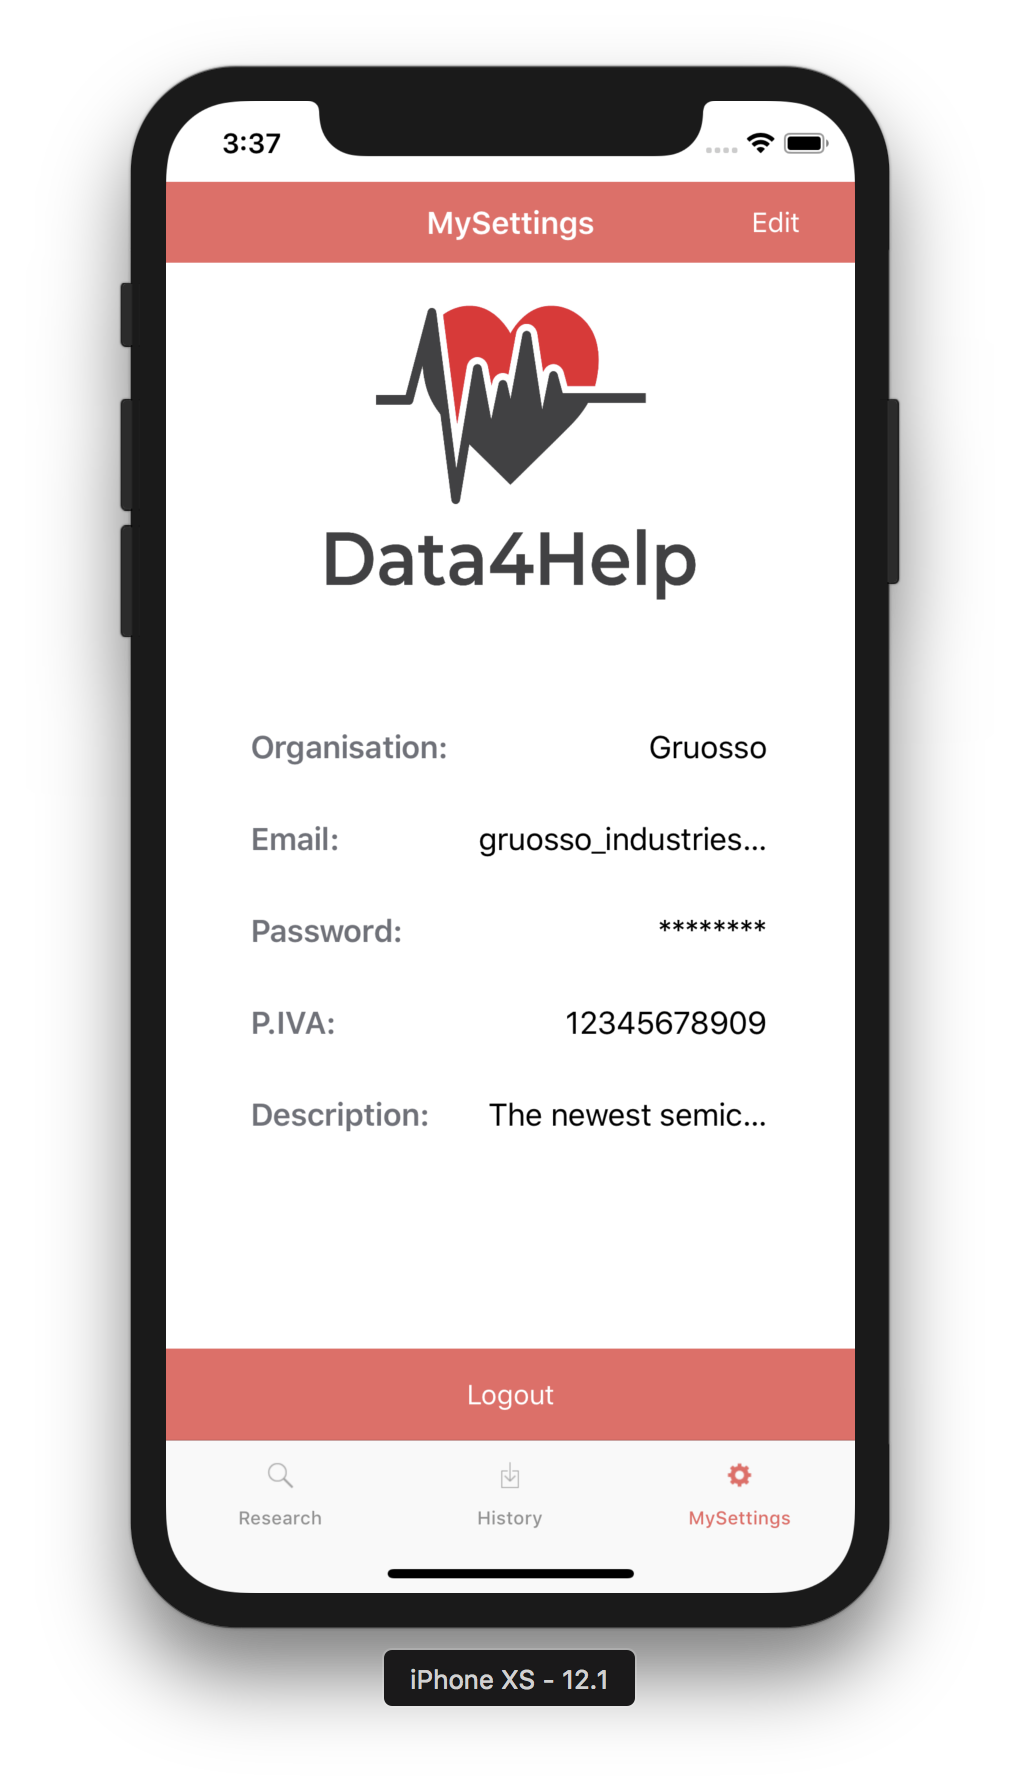
\includegraphics[width=5cm]{images/SimulatorScreenshots/tpsettings.png}}}%
			\qquad
			\subfloat[Edit settings]{{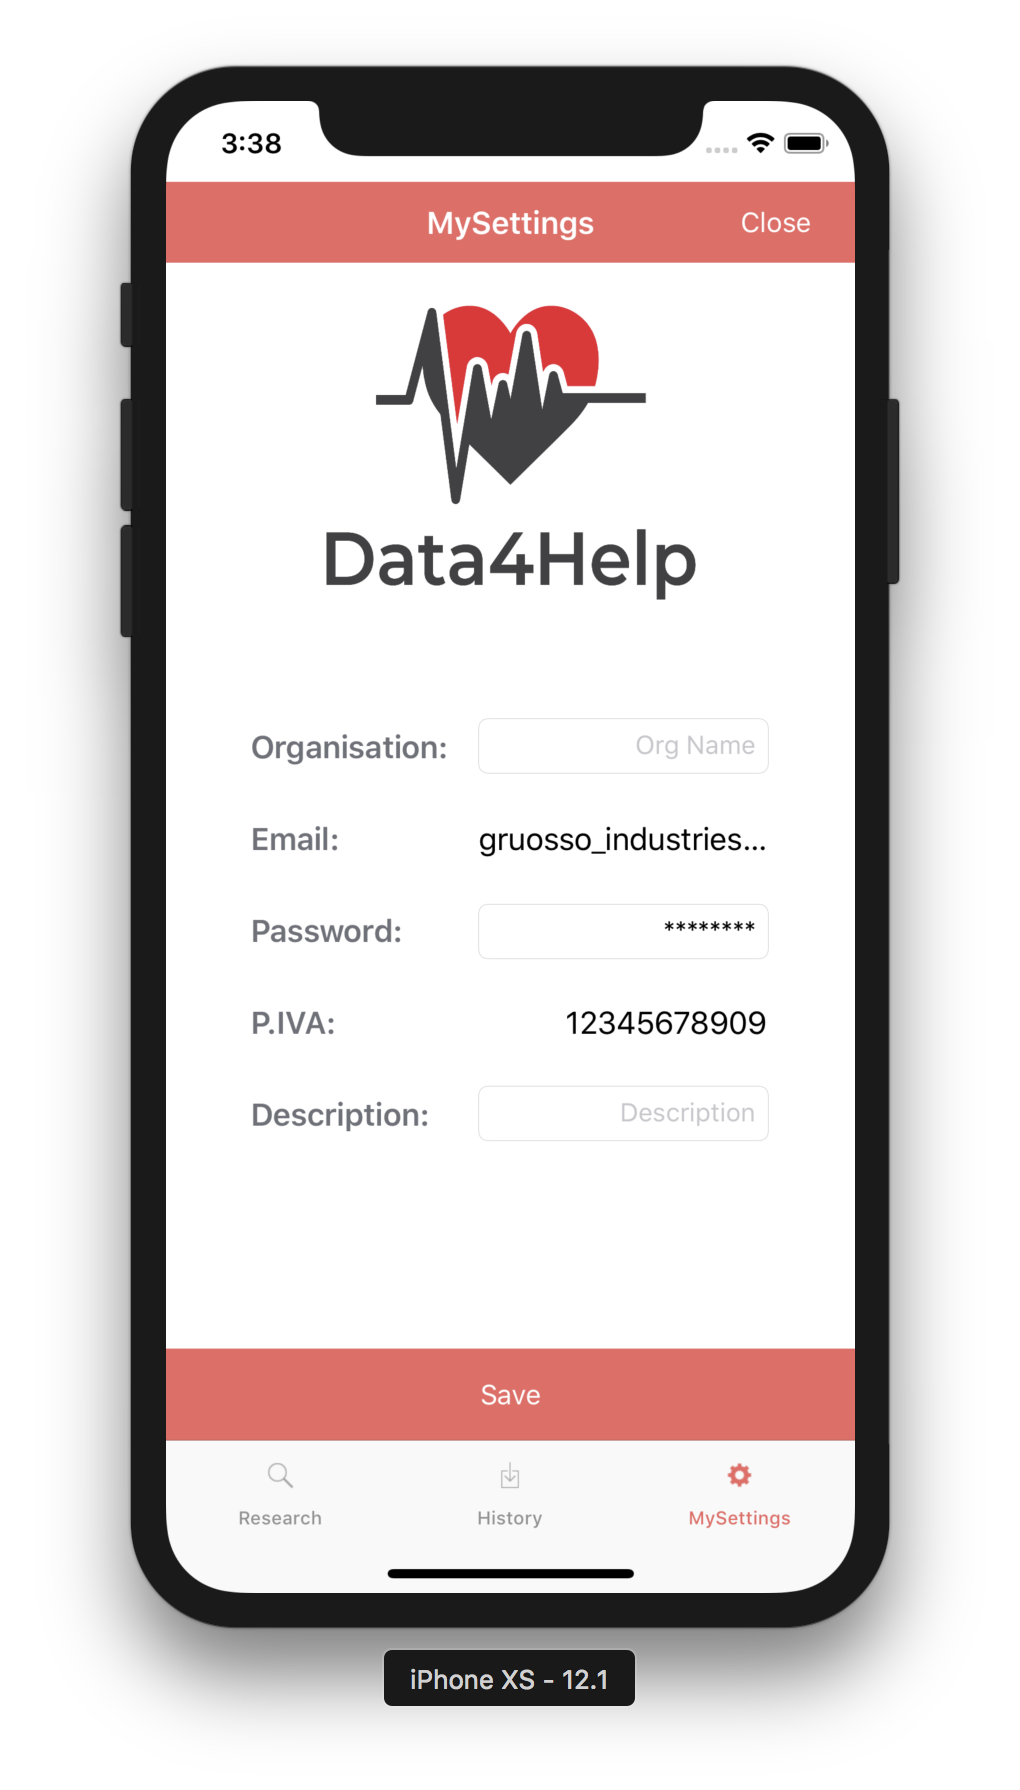
\includegraphics[width=5cm]{images/SimulatorScreenshots/tpeditsettings.png}} }%
			\caption{{\it Third Party} Settings tab screenshots}%
			\label{fig:RequestTab}%
		\end{figure}
		
		{\bf MyHistory controllers}
		\begin{itemize}
			\item {\bf TPRequestsController.swift}: it manages the UITableView containing all the sent requests. It also provides a search bar to easily filter requests based on the receiver name in case of {\it Single Request} or group id in case of {\it Group Request}.
			\item {\bf RequestCellDelegate.swift}: a protocol allowing TPRequestCell and TPGroupRequest classes to call some methods from TPRequestsController.
			\item {\bf PopUpRequestViewController.swift}: a subclass of UIViewController responsible for displaying a popup containing all information related to a specific request. The popup is presented after applying {\it 3D Touch} to a request, both single and group, in the History tab of {\it {\it Third Parties}}.
			
		\end{itemize}
		
		\begin{figure}[H]%
			\centering
			\subfloat[MyHistory view]{{\includegraphics[width=5cm]{images/SimulatorScreenshots/history.png}}}%
			\qquad
			\subfloat[PopUp view]{{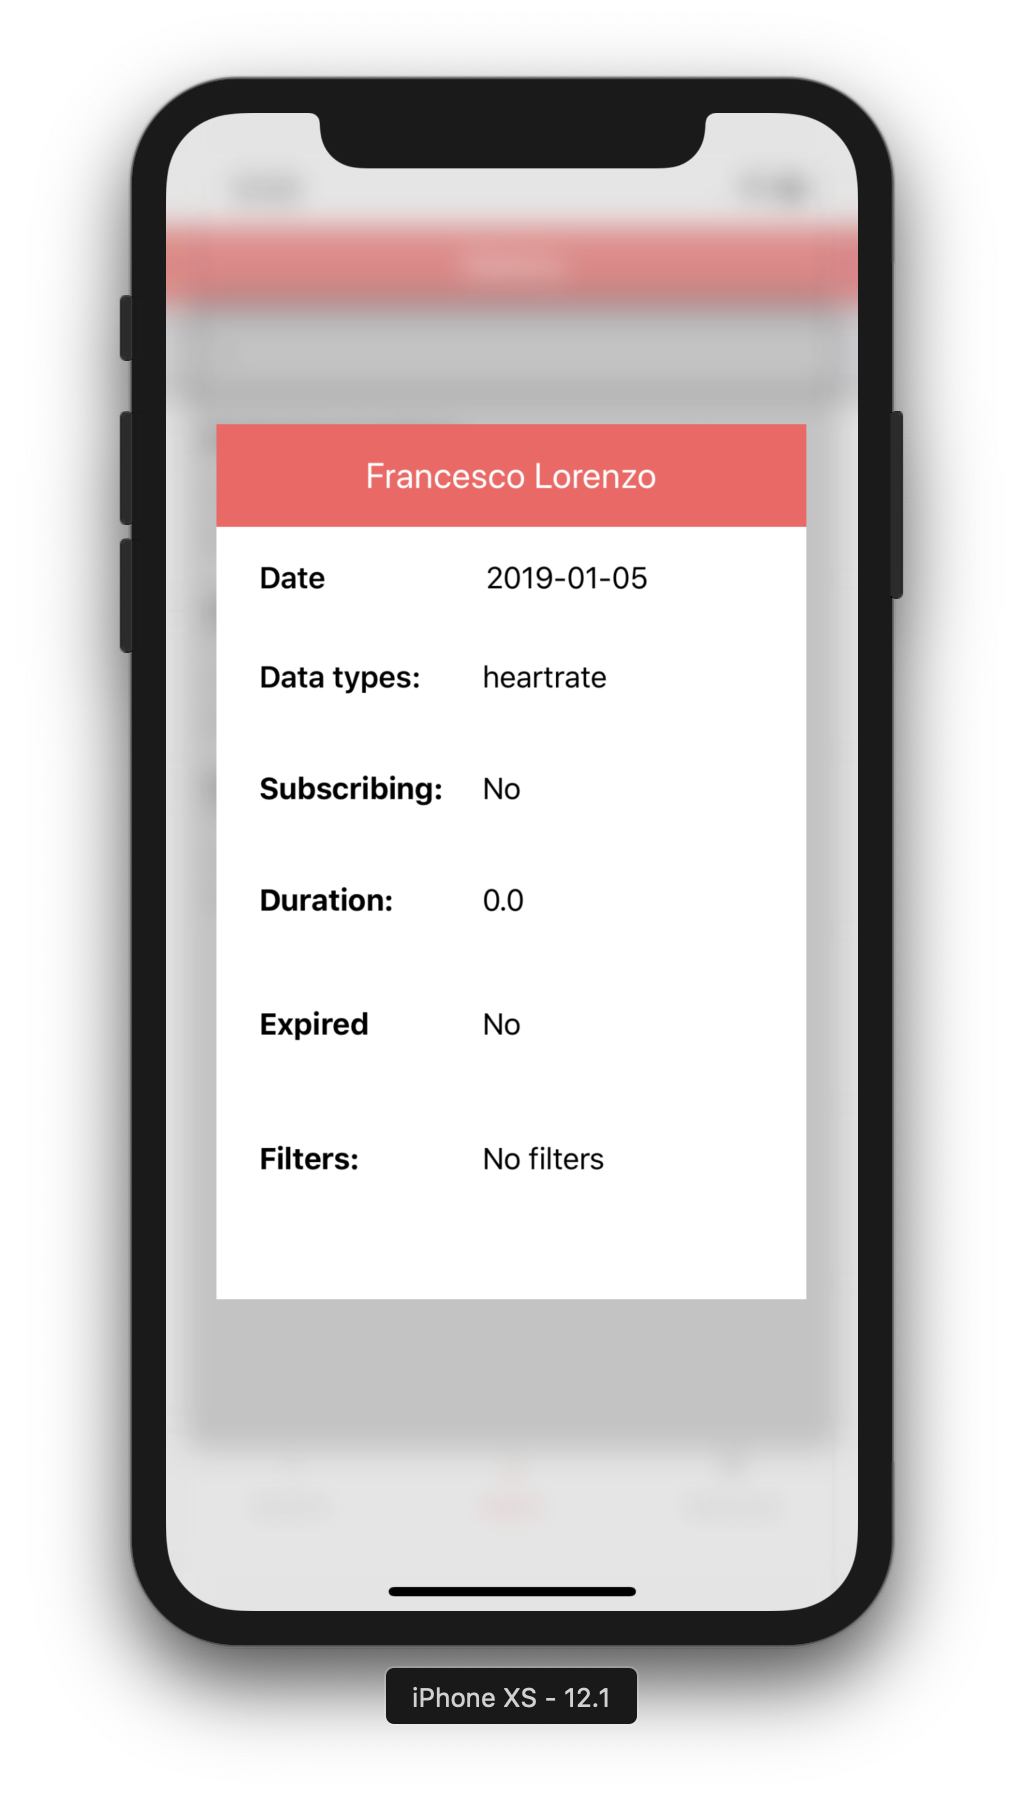
\includegraphics[width=5cm]{images/SimulatorScreenshots/popup.png}} }%
			\caption{MyHistory tab screenshots}%
			\label{fig:RequestTab}%
		\end{figure}
		
	}
	\noindent
	{\bf Health Controllers} \newline
	This group gathers all controllers responsible for interacting with the Healthkit framework and for enabling {\it AutomatedSOS}.
	\begin{itemize}
		\item The {\bf DataManager} class is a Singleton controller class responsible for interacting with HealthKit. This class is at the core of {\it Data4Help} as it is essential to enable features such as Health Monitoring and {\it AutomatedSOS}.
		A unique Healthstore object is kept in order to retrieve all health data from the user\textsc{\char13}s device.
		Once a {\it {\it Single User}} has logged into his account, after having requested his authorization, the DataManager enables background delivery for data from the Health app and imports it as soon as it is produced. All newly imported data is stored into the local CoreData Storage in order to be immediately retrieved when required and to be later sent to the server. As soon as a new health sample is imported it is handled by an appropriate function according to its type: Quantity, Category and Correlation samples. The table below defines all imported types of data and their measurement unit.
		
		\renewcommand*{\arraystretch}{1.4}
		\begin{longtable}{| p{4 cm} | p{4 cm} | p{2 cm} |} \hline
			{\bf Health data} & {\bf Type}  & {\bf Unit} \\ \hline
			Heart Rate & HKQuantitySample & count/min \\ \hline
			Blood pressure & HKCorrelationSample & mmHg \\ \hline
			Steps & HKQuantitySample & count \\ \hline
			Standing Hours & HKCorrelationSample & hours \\ \hline
			Distance Walking Running & HKQuantitySample & miles \\ \hline
			Active Energy Burned & HKQuantitySample & kiloCalories \\ \hline
			Weight & HKQuantitySample & pounds \\ \hline
			Height & HKQuantitySample & feet \\ \hline
		\end{longtable}
		
		The controller also to retrieves from the healthstore the user\textsc{\char13}s biological sex, stored as an HKCharacteristicType, and sends it to the application server together with the information manually input by the user.
		By setting an appropriate timer, the DataManager periodically sends to the server application a message containing all newly imported data. The period is set to one hour in order not to overload the server with requests for every new import.
		If a user decides to enable {\it AutomatedSOS}, this new information is stored by the DataManager. As soon as new data is produced, it is immediately passed to the {\it AutomatedSOS} controller class.
		\item {\bf {\it AutomatedSOS}} is a controller class responsible for analyzing all imported health data and deciding whether a user is in a critical health condition. If this is the case, then it prompts the user to call an ambulance. User confirmation is required to establish the call with the emergency services. 
		This class becomes active only when the user decides to activate the {\it AutomatedSOS} functionality. Enabling this feature can be done also through a quick action by using {\it 3D touch} on the app\textsc{\char13}s icon.
		
		\begin{figure}[H]
			\center
			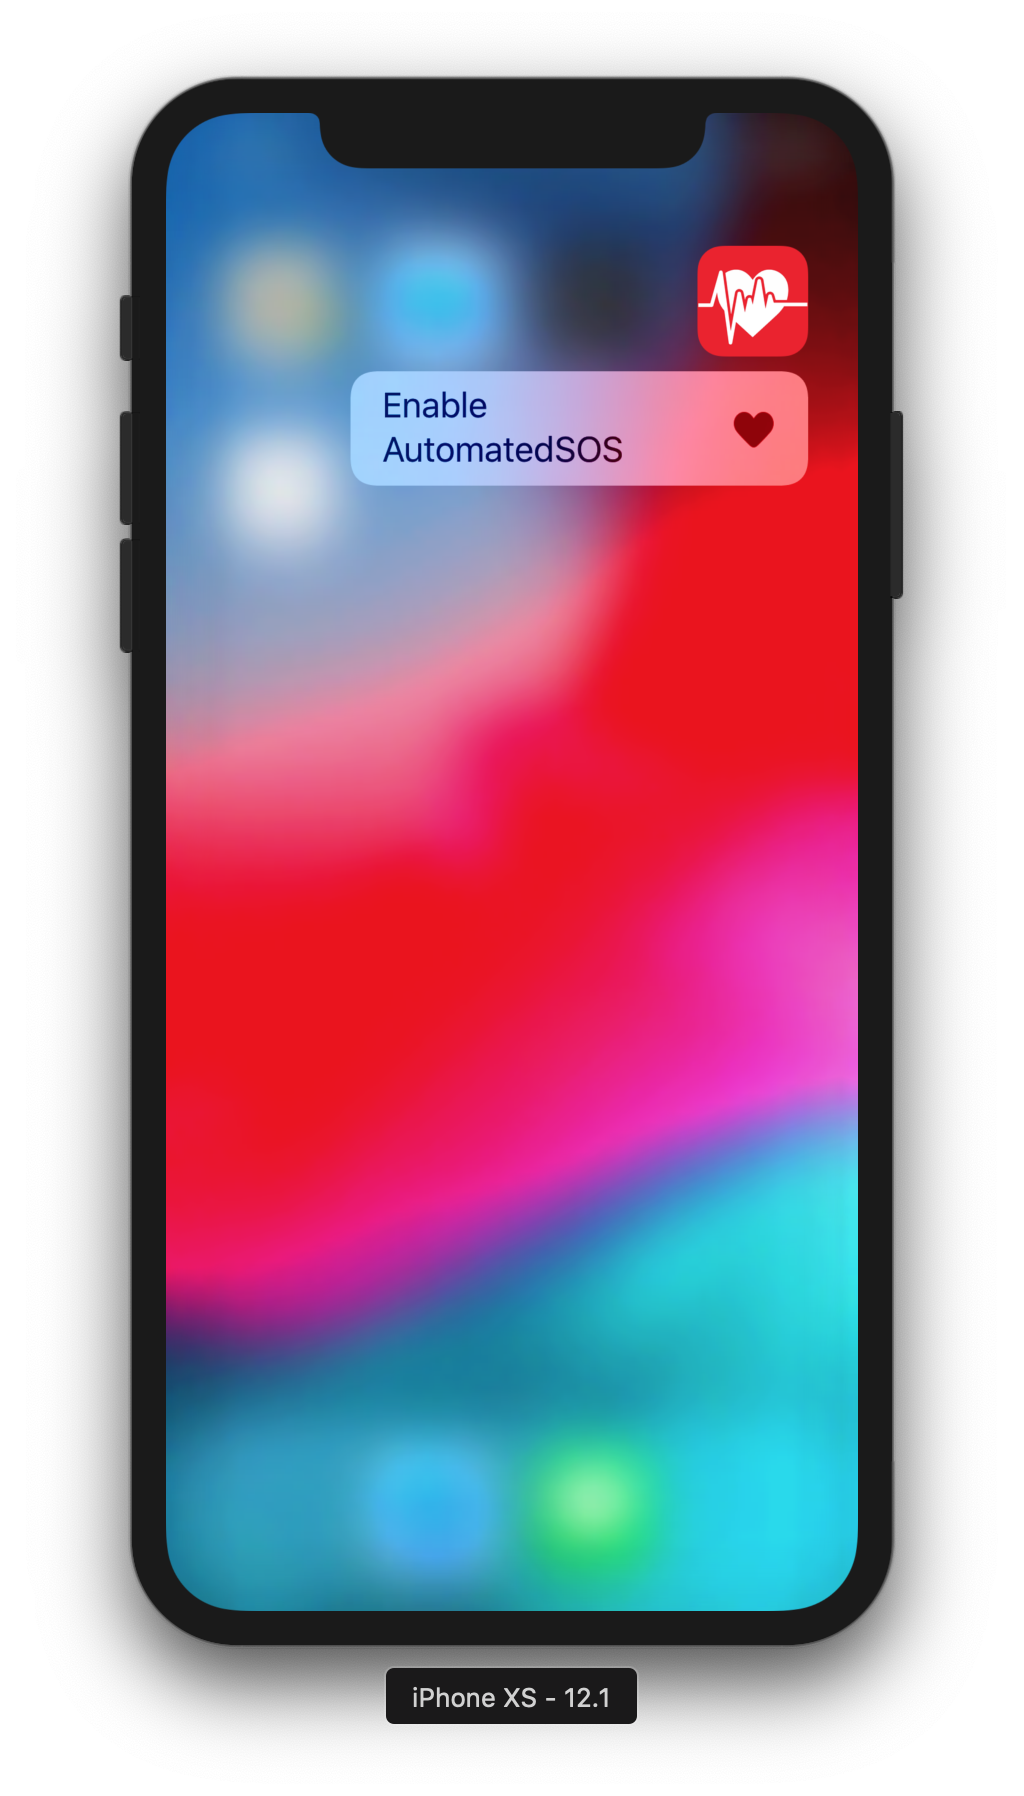
\includegraphics[width=5cm]{SimulatorScreenshots/3DTouch.png}
			\caption{History tab}
			\label{fig:Hist}
		\end{figure}
		
		The parameters evaluated by the class to establish whether a user is in a critical health condition follow the New York Heart Association Guidelines. Specifically, it analyses values of heart rate and blood pressure that define either a Stage 2 Hypertension (with systolic and diastolic pressures respectively above 140 and 90) or a hypotension (with systolic and diastolic pressures respectively below 90 and 60).
		This class can be extended to support other analysis to be performed in order to define a critical health condition.
		As mentioned in the Design Document, all the logic of {\it AutomatedSOS} is located within the Client application in order to evaluate critical conditions immediately and without any delay due to the network.
	\end{itemize}
	
	
	\subsubsection{Models}
	{\bf Data4Help Model} \newline
	{\it Data4Help} Model is a folder containing all the classes used at runtime to represent the state of the application. It presents data structures to keep track of {\it Single} and {\it Group Requests} parameters and content, but also classes for observations and statistics used to draw graphs. Finally Health Parameters and bounds used to perform requests. Most of this objects are thought to be instantiated using the content of network calls responses and thereby present initialisers that accept JSON data.\newline \newline
	\noindent
	{\bf Requests and Responses}\newline
	Under the Model folder are stored all the Request and Response objects used by the NetworkManager. Both Requests and Responses inherit respectively from D4HRequest and D4HResponse allowing the NetworkManager to handle the addition of new requests and responses without changing the code that perform the network calls. Requests and Responses are also organised in a serie of subfolders divided by argument: Request, Data, Settings and Authentication. Regarding Requests they all inherit the method “getParams”, called by the Network Manager to retrieve the JSON encoded parameters to be added into the HTTP request body. Responses on the other hand have an initialiser that allows to build them from the JSON data contained in the HTTP response received by the network manager. The Request and Responses folder presents an additional file called D4HEndopints that contains a data structure that enumerates all the different endpoints reached by the network calls.\newline
	\newline
	\noindent
	{\bf CoreData Model} \newline
	CoreData is a persistence framework that allows to create a relational entity-attribute storage serialized in an SQLite store. In this project it is used as a local storage to store health data imported from Healthkit and the status of {\it AutomatedSOS}. There are three entities to store all the necessary information: “Data”, “BiologicalSex” and “{\it AutomatedSOS}”.
	The first entity is used to store all data imported from Healthkit. It is gathered in chunks as soon as it is produced and periodically sent to the server in order not to overload it with requests. Data entities have three attributes: “type”, “value” and “timestamp”. All stored values correspond to Healthkit objects of time HKSample. The biological sex of a user is store in healthkit as an HKCharacteristicType object being an immutable feature of the user. It is stored in a separate entity and sent to the application server when requested during registration. Finally also the state of {\it AutomatedSOS} is stored permanently in the local storage. All of {\it AutomatedSOS}\textsc{\char13}s logic is developed in the client application so it is essential to store its state and reload it after the app\textsc{\char13}s termination. \newline
	\newline
	\noindent
	{\bf Properties.swift} \newline
	This file contains a struct used to store and manage user\textsc{\char13}s {\it accessToken}, password and email. It allows to easily include the {\it accessToken} in an http header or eventually revoke all credentials in case of logout. It also contains a function called during the logout routine that allows to perform a segue back to the login view. User\textsc{\char13}s password and email are persistently stored using UserDefaults in order to perform an automatic login in case the user closed the app without explicitely logging out.
	
	
	
	
	\subsubsection{Utilities}
	{\bf Network Manager.swift} \newline
	Network manager is a support class that defines a series of handy and general purpose methods that use AlamoFire to perform POST and GET request. Network Manager implement a singleton pattern ao that a shared instance of the class is always available everywhere in the application. This choice also fits well with the stateless nature of this component. As already mentioned the Network manager allows to perform network calls from everywhere in the client application and it offer a very generic and expandible structure that easily support the introduction of new requests and  endpoints. \newline
	\newline
	\noindent
	{\bf Storage Manager} \newline
	The Storage Manager is the controller classes devoted to interacting with {\it CoreData}, a persistence framework that allows to create a relational entity-attribute storage serialized in an SQLite store. A local storage in the client application is needed to collect newly imported data from Healthkit used to be displayed to the user or gathered and sent in chunks to the server. The information stored in {\it CoreData} is essentially all health data related to the user and the activation state of {\it AutomatedSOS}. While the imported health data is cached only for a certain period of time, the information about {\it AutomatedSOS} is stored permanently in order to be retrieved after the app\textsc{\char13}s termination.
	This controller is a singleton class and is referenced throughout the whole project whenever new data needs to be stored permanently or retrieved. \newline
	\newline
	\noindent
	{\bf App Delegate} \newline
	The Application Delegate is the class responsible for handling all events related to the application\textsc{\char13}s lifecycle such as when it is launched, when it works in background and foreground and when it terminates.
	When the application is launched for the first time it performs setup operations such as setting up {\it CoreData}, requesting the user\textsc{\char13}s authorization to access Health, initializing {\it AutomatedSOS} and setting up background fetching of health data. It is also responsible for handling quick actions that are set up dynamically during the app\textsc{\char13}s execution. When the app is launched through a quick action, the App delegate is responsible for calling the appropriate handler.
	The Application Delegate follows the Delegation pattern. The core purpose of this pattern is to allow an object to communicate back to its owner in a decoupled way. 
	\newline
	\newline
	\noindent
	
	
	
	\pagebreak
	%%%%%%%%%%%%%%%%%%%%%%%%%%%%Testing%%%%%%%%%%%%%%%%%%%%%%%%%%%%%%%%%%%%%%%%%%%%%%
	\section{Testing}
	Testing has been done following the specifications present in the Design Document. \\
	\linebreak
	For the Backend, two frameworks were used: Jest and Supertest. 
	Jest is a widespread JavaScript testing library with mockup functionalities, high-level abstractions, various types of assertions and offers clean code structure.
	Supertest is a library used mainly for Integration testing, and provides an easy way to test Express endpoints and make HTTP assertions.
	Testing code is located in the tests folder, recreating the source code structure inside it.
	
	%%%%%%%%%%% UNIT TESTING %%%%%%%%%%%%%%%%
	\subsection{Unit Testing}
	\subsubsection{Backend}
	Unit Testing in the backend is limited, as there are few modules that have specific functions not relying on external components, and implementing meaningful algorithms. 
	The most suitable and critical module that needed unit testing was schemas.js, defining the schemas of requests, and was thoroughly tested. To properly perform Unit Testing, the module was directly tested, not relying on its function as a middleware. 
	Same properties (like password and email) were tested for one schema, as nothing changes for the others. The test cases performed are the following:
	\renewcommand*{\arraystretch}{1.4}
	\begin{longtable}{| p{3 cm} | p{5 cm} | p{3 cm} |} \hline
		{\bf Schema} & {\bf Test Description} & {\bf Desired Output} \\ \hline
		{\it Single User} registration & \begin{itemize}[nolistsep]
			\item[$-$] Object respecting the schema
		\end{itemize}
		& Error is null \\ \hline
		{\it Single User} registration & \begin{itemize}[nolistsep]
			\item[$-$] Missing password
			\item[$-$] Password length isn\textsc{\char13}t 8 characters
			\item[$-$] Password not being a string
		\end{itemize}
		& Validation error \\ \hline
		{\it Single User} registration & \begin{itemize}[nolistsep]
			\item[$-$] Missing email
			\item[$-$] Email too long
			\item[$-$] Wrong regex
			\item[$-$] Email not being a string
		\end{itemize}
		& Validation error \\ \hline
		{\it Single User} registration & \begin{itemize}[nolistsep]
			\item[$-$] Missing FC
			\item[$-$] FC length isn\textsc{\char13}t 16 characters
			\item[$-$] FC not being a string
		\end{itemize}
		& Validation error \\ \hline
		{\it Single User} registration & \begin{itemize}[nolistsep]
			\item[$-$] Missing full name
			\item[$-$] Full name too long
			\item[$-$] Full name not being a string
		\end{itemize}
		& Validation error \\ \hline
		{\it Single User} registration & \begin{itemize}[nolistsep]
			\item[$-$] Missing birthdate
			\item[$-$] Birthdate not a date
			\item[$-$] Birthdate not respecting ISO specifications Validation error
		\end{itemize}
		& Validation error \\ \hline
		{\it Single User} registration & \begin{itemize}[nolistsep]
			\item[$-$] Missing sex
			\item[$-$] Sex not “M” or “F”
		\end{itemize}
		& Validation error \\ \hline
		{\it Third Party} registration & \begin{itemize}[nolistsep]
			\item[$-$] Object respecting the schema
		\end{itemize}
		& Error is null \\ \hline
		{\it Third Party} registration & \begin{itemize}[nolistsep]
			\item[$-$] Missing P.IVA
			\item[$-$] P.IVA length isn\textsc{\char13}t 11 characters
			\item[$-$] P.IVA is not a string
		\end{itemize}
		& Validation error \\ \hline
		{\it Third Party} registration & \begin{itemize}[nolistsep]
			\item[$-$] Missing company name
			\item[$-$] Company name longer than 20 characters
			\item[$-$] Company name not being a string
		\end{itemize}
		& Validation error \\ \hline
		{\it Third Party} registration & \begin{itemize}[nolistsep]
			\item[$-$] Company description not being a string
		\end{itemize}
		& Validation error \\ \hline
		Login & \begin{itemize}
			\item[$-$] Object respecting the schema
		\end{itemize}
		& Error is null \\ \hline
		{\it Single User} settings & \begin{itemize}[nolistsep]
			\item[$-$] Object respecting the schema
		\end{itemize}
		& Error is null \\ \hline
		{\it Third Party} settings & \begin{itemize}[nolistsep]
			\item[$-$] Object respecting the schema
		\end{itemize}
		& Error is null \\ \hline
		Import data & \begin{itemize}
			\item[$-$] Object respecting the schema
		\end{itemize}
		& Error is null \\ \hline
		Import data & \begin{itemize}[nolistsep]
			\item[$-$] Data type array missing
			\item[$-$] Invalid data type in the array
			\item[$-$] Length not matching the value array
		\end{itemize}
		& Validation Error \\ \hline
		Import data & \begin{itemize}[nolistsep]
			\item[$-$] Value array missing
			\item[$-$] Invalid value in the array
			\item[$-$] Length not matching the data type array
		\end{itemize}
		& Validation Error \\ \hline
		Import data & \begin{itemize}[nolistsep]
			\item[$-$] Timestamp array missing
			\item[$-$] Invalid value in the array
			\item[$-$] Length not matching the value array
		\end{itemize}
		& Validation Error \\ \hline
		Statistics & \begin{itemize}[nolistsep]
			\item[$-$] Object respecting the schema
		\end{itemize}
		& Error is null \\ \hline
		Send a single request & \begin{itemize}[nolistsep]
			\item[$-$] Object respecting the schema
		\end{itemize}
		& Error is null \\ \hline
		Send a single request & \begin{itemize}[nolistsep]
			\item[$-$] Subscription is not a boolean
		\end{itemize}
		& Validation error \\ \hline
		Send a single request & \begin{itemize}[nolistsep]
			\item[$-$] Duration is not an integer
			\item[$-$] Duration is present if subscribing is false
		\end{itemize}
		& Validation error \\ \hline
		Send a group request & \begin{itemize}[nolistsep]
			\item[$-$] Object respecting the schema
		\end{itemize}
		& Error is null \\ \hline
		Send a group request & \begin{itemize}[nolistsep]
			\item[$-$] Missing parameters array
			\item[$-$] Invalid value in the array
			\item[$-$] Length not matching the bounds array
		\end{itemize}
		& Validation error \\ \hline
		Send a group request & \begin{itemize}[nolistsep]
			\item[$-$] Missing parameters array
			\item[$-$] Invalid value in the array for lowerbound
			\item[$-$] Length not matching the bounds array
		\end{itemize}
		& Validation error \\ \hline
		Accept a request & \begin{itemize}[nolistsep]
			\item[$-$] Object respecting the schema
		\end{itemize}
		& Error is null \\ \hline
		Accept a request & \begin{itemize}[nolistsep]
			\item[$-$] Missing ReqID
			\item[$-$] ReqID not being an integer
		\end{itemize}
		& Validation error \\ \hline
		Accept a request & \begin{itemize}[nolistsep]
			\item[$-$] Missing choice
			\item[$-$] Choice not being a boolean
		\end{itemize}
		& Validation error \\ \hline
		Download a request & \begin{itemize}[nolistsep]
			\item[$-$] Object respecting the schema
		\end{itemize}
		& Error is null \\ \hline
		
		\caption{Unit testing test cases}	
	\end{longtable}
	
	%%%%%%%%%%% INTEGRATION TESTING %%%%%%%%%%%%%%%%
	\subsection{Integration Testing}
	\subsubsection{Backend}
	As previously explained, integration testing has been done using Supertest as framework. The core of the backend, the Express app, has been tested endpoint by endpoint from when a request is received up to when the response is sent (and received by Supertest), together with all its dependencies. In particular, in order to maintain production and development separate, a local PostgreSQL database was created, and all its data is completely erased after every test suite, so tests don\textsc{\char13}t interfere with each other. 
	All integration tests do not check for syntactic mistakes, as they were already tested through Unit Testing, but rather for semantic errors.
	The test cases performed are the following:
	
	
	\renewcommand*{\arraystretch}{1.4}
	\begin{longtable}{| p{3 cm} | p{4 cm} | p{4 cm} |} \hline
		{\bf Endpoint} & {\bf Test Description} & {\bf Desired output} \\ \hline
		/auth/reg/single & Valid request is provided & HTTP 200: Database contains the new user, activation mail is sent \\ \hline
		/auth/reg/single & Register a user who\textsc{\char13}s already registered & HTTP 403: Account is not created \\ \hline
		/auth/reg/tp & Valid request is provided & HTTP 200: Database contains the new user, activation mail is sent \\ \hline
		/auth/reg/tp & Register a user who\textsc{\char13}s already registered & HTTP 403: Account is not created \\ \hline
		/auth/activ & Activate a registered account providing a correct token & HTTP 200: Account is activated in the database \\ \hline
		/auth/activ & Activate an already activated account & HTTP 403: Account is not activated \\ \hline
		/auth/activ & Activate a non existing account & HTTP 401: Account is not activated, can\textsc{\char13}t access the resource \\ \hline
		/auth/login & Login using correct credentials for an existing account & HTTP 200: Login successful, authToken in the response \\ \hline
		/auth/login & Login with an invalid email & HTTP 401: Login failed, can\textsc{\char13}t access the resource \\ \hline
		/auth/login & Login in a non activated account & HTTP 401: Login failed, can\textsc{\char13}t access the resource \\ \hline
		/auth/login & Login with wrong password & HTTP 401: Login failed, can\textsc{\char13}t access the resource \\ \hline
		/data/upload & Upload data of a logged user & HTTP 200: Data is now present in the database \\ \hline
		/data/upload & Upload data of a non logged user & HTTP 401: Can\textsc{\char13}t access the resource \\ \hline
		/data/upload & Upload data which in part was already present & HTTP 200: Only new data is imported \\ \hline
		/data/stats/avg & Retrieve statistics of a logged user with data of other users already present in the db & HTTP 200: Statistics retrieved in the response, taking into account also other users \\ \hline
		/req/tp/sendSingle & Send a single request by a logged {\it Third Party} & HTTP 200: Request is now present in the database \\ \hline
		/req/tp/sendSingle & Send a request to a non existing user & HTTP 403: Can\textsc{\char13}t find the user, request is not inserted in the db \\ \hline
		/req/tp/sendSingle & Send a request to an user who has a pending request already & HTTP 403: Can\textsc{\char13}t send the request, db is not updated \\ \hline
		/req/tp/sendGroup & Send a group request by a logged {\it Third Party} & HTTP 200: Request is now present in the database \\ \hline
		/req/single/choice & Accept and refuse an existing pending request & HTTP 200: Request is updated in the database \\ \hline
		/req/single/choice & Accept a non pending request & HTTP 403: Can\textsc{\char13}t accept a non pending request \\ \hline
		/req/single/choice & Accept a non existing request & HTTP 403: Can\textsc{\char13}t accept a non existing request \\ \hline
		/req/single/list & Retrieve list of requests of a {\it Single User} & HTTP 200: Response contains all the requests to the user \\ \hline
		/req/tp/list & Retrieve list of requests of a {\it Third Party} & HTTP 200: Response contains all the requests (single and group) of the user \\ \hline
		/sub/endSingle & Terminate an ongoing subscription (by both {\it Single User}s and {\it Third Parties}) & HTTP 200: Subscribing is now false in the database, subscription is ended \\ \hline
		/sub/endSingle & Terminate an expired subscription & HTTP 403: Subscription was already expired \\ \hline
		/sub/endSingle & Terminate a subscription of a non accepted request & HTTP 403: Can\textsc{\char13}t terminate the subscription \\ \hline
		/sub/endGroup & Terminate an ongoing subscription to a group request by the sender {\it Third Party} & HTTP 200: Subscribing is now false in the database, subscription is ended \\ \hline
		/sub/endGroup & Terminate an expired subscription & HTTP 403: Subscription was already expired \\ \hline
		/sub/endGroup & Terminate a subscription of a non accepted request & HTTP 403: Can\textsc{\char13}t terminate the subscription \\ \hline
		/tp/downloadSingle & Download data of an accepted single request & HTTP 200: Response contains data of the target user \\ \hline
		/tp/downloadSingle & Download data of a non accepted request & HTTP 403: Can\textsc{\char13}t download the data \\ \hline
		/tp/downloadSingle & Download data of a non existing request & HTTP 403: Request does not exist \\ \hline
		/tp/downloadGroup & Download data of a group request & HTTP 200: Response contains anonymised data requested \\ \hline
		/tp/downloadGroup & Download data of a non existing request & HTTP 403: Request does not exist \\ \hline
		/tp/downloadGroup & Download data of a request that doesn\textsc{\char13}t match the 1000 users constraint & HTTP 403: Not enough users match the Search Parameters \\ \hline
		/settings/single/info & Update settings of a logged users & HTTP 200: Settings are updated in the database \\ \hline
		/settings/single/info & Retrieve settings of a logged users & HTTP 200: Response contains the settings \\ \hline
		/settings/single/info & Update settings of a non logged users & HTTP 401: Can\textsc{\char13}t access the resource \\ \hline
		/settings/single/info & Update settings of another user & HTTP 401: Can\textsc{\char13}t access the resource \\ \hline
		/settings/tp/info & Update settings of a logged users & HTTP 200: Settings are updated in the database \\ \hline
		/settings/tp/info & Retrieve settings of a logged users & HTTP 200: Response contains the settings \\ \hline
		/settings/tp/info & Update settings of a non logged users & HTTP 401: Can\textsc{\char13}t access the resource \\ \hline
		/settings/tp/info & Update settings of another user & HTTP 401: Can\textsc{\char13}t access the resource \\ \hline
		\caption{Integration Testing Test cases}	
	\end{longtable}
	
	\subsection{System Testing}
	System testing is essential to test the system's compliance with the specified requirements. The test cases described in the following table allow us to test the interaction between Data4Help's frontend and backend, verify the correctness of all services and receive feedback through the user interface.
	\begin{longtable}{| p{3 cm} | p{4 cm} | p{4 cm} |} \hline
		{\bf Schema} & {\bf Test Description} & {\bf Desired output} \\ \hline
		Register a single user & \begin{itemize}[nolistsep]
			\item[$-$] Insert valid information
		\end{itemize}
		& \begin{itemize}[nolistsep]
			\item[$-$] Go back to the Login View
			\item[$-$] Receive an activation link via email
		\end{itemize} \\ \hline
		Register a single user & \begin{itemize}[nolistsep]
			\item[$-$] Send an empty request
		\end{itemize}
		& \begin{itemize}[nolistsep]
			\item[$-$] Receive an error alert
		\end{itemize} \\ \hline
		Register a single user & \begin{itemize}[nolistsep]
			\item[$-$] Insert invalid information (birthdate, password or CF malformed)
		\end{itemize}
		& \begin{itemize}[nolistsep]
			\item[$-$] Receive an error alert
		\end{itemize} \\ \hline
		Register a third party & \begin{itemize}[nolistsep]
			\item[$-$] Insert valid information
		\end{itemize}
		& \begin{itemize}[nolistsep]
			\item[$-$] Go back to the Login View
			\item[$-$] Receive an activation link via email
		\end{itemize} \\ \hline
		Register a third party & \begin{itemize}[nolistsep]
			\item[$-$] Send an empty request
		\end{itemize}
		& \begin{itemize}[nolistsep]
			\item[$-$] Receive an error alert
		\end{itemize} \\ \hline
		Register a third party & \begin{itemize}[nolistsep]
			\item[$-$] Insert invalid information (P.IVA, or password malformatted)
		\end{itemize}
		& \begin{itemize}[nolistsep]
			\item[$-$] Receive an error alert
		\end{itemize} \\ \hline
		Login & \begin{itemize}[nolistsep]
			\item[$-$] Insert valid credentials
		\end{itemize}
		& \begin{itemize}[nolistsep]
			\item[$-$] Enter logged-in view
		\end{itemize} \\ \hline
		Login & \begin{itemize}[nolistsep]
			\item[$-$] Send an empty request
		\end{itemize}
		& \begin{itemize}[nolistsep]
			\item[$-$] Receive an error alert
		\end{itemize} \\ \hline
		Login & \begin{itemize}[nolistsep]
			\item[$-$] Insert invalid credentials
		\end{itemize}
		& \begin{itemize}[nolistsep]
			\item[$-$] Receive an error alert
		\end{itemize} \\ \hline
		Login & \begin{itemize}[nolistsep]
			\item[$-$] Insert credentials of an account that has not been activated
		\end{itemize}
		& \begin{itemize}[nolistsep]
			\item[$-$] Receive an error alert
		\end{itemize} \\ \hline
		Create a Single Request & \begin{itemize}[nolistsep]
			\item[$-$] Insert valid email or CF and select some datatypes
		\end{itemize}
		& \begin{itemize}[nolistsep]
			\item[$-$] Receive an alert confirming the request has been sent
		\end{itemize} \\ \hline
		Create a Single Request & \begin{itemize}[nolistsep]
			\item[$-$] Insert invalid email or CF
		\end{itemize}
		& \begin{itemize}[nolistsep]
			\item[$-$] Receive an error alert
		\end{itemize} \\ \hline
		Create a Single Request & \begin{itemize}[nolistsep]
			\item[$-$] Insert valid email or CF but empty list of datatypes
		\end{itemize}
		& \begin{itemize}[nolistsep]
			\item[$-$] Receive an error alert
		\end{itemize} \\ \hline
		Create a Group Request & \begin{itemize}[nolistsep]
			\item[$-$] Select filters and datatypes
		\end{itemize}
		& \begin{itemize}[nolistsep]
			\item[$-$] Receive an alert confirming the request has been sent
		\end{itemize} \\ \hline
		Create a Group Request & \begin{itemize}[nolistsep]
			\item[$-$] Insert empty list of datatypes
		\end{itemize}
		& \begin{itemize}[nolistsep]
			\item[$-$] Receive an error alert
		\end{itemize} \\ \hline
		Refresh History tab & \begin{itemize}[nolistsep]
			\item[$-$] Open History tab to check current requests
			\item[$-$] Create a new single or group request
			\item[$-$] Open History tab
			\item[$-$] Pull to refresh 
		\end{itemize}
		& \begin{itemize}[nolistsep]
			\item[$-$] Receive an updated list of requests with the newly created one
		\end{itemize} \\ \hline
		Edit Third Party Settings & \begin{itemize}[nolistsep]
			\item[$-$] Edit Settings with valid information and press save
		\end{itemize}
		& \begin{itemize}[nolistsep]
			\item[$-$] Edits are saved correctly and editing mode is closed
		\end{itemize} \\ \hline
		Edit Third Party Settings & \begin{itemize}[nolistsep]
			\item[$-$] Edit settings with invalid information
		\end{itemize}
		& \begin{itemize}[nolistsep]
			\item[$-$] Receive an error alert
		\end{itemize} \\ \hline
		Update MyHealth View & \begin{itemize}[nolistsep]
			\item[$-$] Tap charts for update after adding new data to Health
		\end{itemize}
		& \begin{itemize}[nolistsep]
			\item[$-$] See updated Charts
		\end{itemize} \\ \hline
		Refresh MyFollowers tab & \begin{itemize}[nolistsep]
			\item[$-$] Open MyFollowers tab to check current requests
			\item[$-$] Create a new single request from a third party account
			\item[$-$] Pull to refresh 
		\end{itemize}
		& \begin{itemize}[nolistsep]
			\item[$-$] Receive an updated list of requests with the newly created one with status pending
		\end{itemize} \\ \hline
		Accept single request & \begin{itemize}[nolistsep]
			\item[$-$] Send a single request to the user from a third party
			\item[$-$] Select accept button on a pending single request
		\end{itemize}
		& \begin{itemize}[nolistsep]
			\item[$-$] The request will appear in the Accepted Requests section of the MyFollowers tab
			\item[$-$] The request will appear in the Accepted Requests section of the History tab of the third party sending it
		\end{itemize} \\ \hline
		Refuse single request & \begin{itemize}[nolistsep]
			\item[$-$] Send a single request to the user from a third party account
			\item[$-$] Select refuse button on a pending single request
		\end{itemize}
		& \begin{itemize}[nolistsep]
			\item[$-$] The request will appear in the Refused Requests section of the MyFollowers tab
			\item[$-$] The request will appear in the Refused Requests section of the History tab of the third party sending it
		\end{itemize} \\ \hline
		Activate AutomatedSOS & \begin{itemize}[nolistsep]
			\item[$-$] Enable AutomatedSOS switch in MyHealth
			\item[$-$] Add low heart rate sample in Health for testing
		\end{itemize}
		& \begin{itemize}[nolistsep]
			\item[$-$] Receive an alert to call an ambulance as soon as the sample is added
		\end{itemize} \\ \hline
		Activate AutomatedSOS & \begin{itemize}[nolistsep]
			\item[$-$] Disable AutomatedSOS switch
			\item[$-$] Add low heart rate sample in Health for testing
		\end{itemize}
		& \begin{itemize}[nolistsep]
			\item[$-$] No alert to call an ambulance is received when the sample is added
		\end{itemize} \\ \hline
		Enable AutomatedSOS & \begin{itemize}[nolistsep]
			\item[$-$] Close app
			\item[$-$] Press app with 3DTouch and select “Enable AutomatedSOS”
		\end{itemize}
		& \begin{itemize}[nolistsep]
			\item[$-$] App opens and AutomatedSOS switch is on
		\end{itemize} \\ \hline
		Edit Single User Settings & \begin{itemize}[nolistsep]
			\item[$-$] Edit Settings with valid information and press save
		\end{itemize}
		& \begin{itemize}[nolistsep]
			\item[$-$] Edits are saved correctly and editing mode is closed
		\end{itemize} \\ \hline
		Edit Single User Settings & \begin{itemize}[nolistsep]
			\item[$-$] Edit settings with invalid information
		\end{itemize}
		& \begin{itemize}[nolistsep]
			\item[$-$] Receive an error alert
		\end{itemize} \\ \hline
		\caption{System Testing Test Cases}
	\end{longtable}
	
	\pagebreak
	%%%%%%%%%%%%%%%%%%%%%%%%%%%%%%%%%%%%%%%%%%%%%%%%%%%%%%%%%%%%%%%%%%%%%%%%%%%%%%%%%%%%%
	%Testing
	\section{Installation}
	\subsection{Preliminary Operations}
	The following Installation procedure is valid for MacOS. Please contact us for troubleshooting.
	The Backend can be setup for other OS, but some steps might be different, please refer to online documentation if needed.
	The Frontend can only be setup for MacOS, as XCode is available only for said environment.\\
	\linebreak
	First of all you need to clone our GitHub repository.
	\begin{enumerate}
		\item Make sure you have git client installed.
		\item Open a shell and change directory to where you want to install our repository.
		\item Type “git clone \href{https://github.com/iPhra/LorenzoMolteniNegri.git}{https://github.com/iPhra/LorenzoMolteniNegri.git}”
	\end{enumerate}
	
	\subsection{Backend}
	To access the Backend source code, and modify it, you need Node.js and an IDE for JavaScript.
	
	\begin{enumerate}
		\item Download the latest LTS release of Node.js from \href{https://nodejs.org/en/download/}{https://nodejs.org/en/download/}.
		\item Download a JavaScript IDE: we recommend WebStorm as it\textsc{\char13}s the one used for development, but other options like Visual Studio Code are fine.
		\item Open a shell and head to /LorenzoMolteniNegri/Backend/NodeJS.
		\item Type “npm install” to install all dependencies. 
		\item You can now run the Backend server locally by either:
		\begin{itemize}
			\item Opening a shell in /LorenzoMolteniNegri/Backend/NodeJS and typing “npm start” (recommended).
			\item Opening your IDE and creating a new Project selecting /LorenzoMolteniNegri/Backend/NodeJS as root, then creating a script to run it. Please refer to the documentation provided for your IDE, make sure to select bin/www.js as the executable to run.
		\end{itemize}
	\end{enumerate}
	To run all tests you need to install a local PostgreSQL database. 
	Follow the steps mentioned in this guide \href{https://www.codementor.io/engineerapart/getting-started-with-postgresql-on-mac-osx-are8jcopb}{https://www.codementor.io/engineerapart/getting-started-with-postgresql-on-mac-osx-are8jcopb} for what concerns installing Postgres through Homebrew, creating a user and creating the database.
	Once the database is up and running, recreate the DB schema provided in this documentation using a SQL client of your choice. For SQLWorkbenchJ, to access and modify the database, follow these steps:
	\begin{enumerate}
		\item In the Select Connection window, choose the Driver for PostgreSQL among those available.
		\item Use this url: “jdbc:postgresql://localhost/yourdbname”. yourdbname should be the name you used when you created the local database.
		\item Username should be the one used when creating your user in the aforementioned guide.
		\item Leave all other options default, and connect to the database.
		\item You can now recreate our schema by using Statement windows to type SQL commands.
	\end{enumerate}
	
	When the database is ready, open Terminal and head to /LorenzoMolteniNegri/Backend/NodeJS, you can now run all tests by typing “npm test”.
	
	\subsection{Frontend}
	To access the frontend\textsc{\char13}s source code you must have XCode installed and do the following steps:
	\begin{enumerate}
		\item In XCode open the Xcode workspace file of {\it Data4Help} located in /LorenzoMolteniNegri/iOS/Data4Help/
		\item In the project\textsc{\char13}s General tab insert valid Developer Account credentials in the “Team” field.
		\item To build the project you must select a destination under $Product \rightarrow Destination$. You can either:
		\begin{tasks}
			\task Select an iOS Simulator. We recommend using an iPhone XS simulator to take advantage of the wide screen and latest capabilities.
			\task Select your personal device after having connected it to the USB port. Please be sure to be running iOS 8.0 or a later version. We recommend running the latest version of iOS.
		\end{tasks}
		\item Run the application. If the destination is your personal device an error will appear after having installed the app for the first time. The error appears because the Developer App certificate for your account must be trusted on your device. To remove it proceed as follows:
		\begin{tasks}
			\task In your device go to Settings.
			\task In Settings navigate to $General\rightarrow Profiles \& Management$ and select your Developer App certificate to trust it.
		\end{tasks}
		\item Open the app.
	\end{enumerate}
	
	\pagebreak
	%%%%%%%%%%%%%%%%%%%%%%%%%%%%%%%%%%%%%%%%%%%%%%%%%%%%%%%%%%%%%%%%%%%%%%%%%%%%%%%%%%%%%
	%Efforts
	\section{Future developments}
	Some future developments have already been planned, but are not included in this first release due to either lack of time or financial limitations. In particular, the motivations are:
	
	\begin{itemize}
		\item {\bf Nginx proxy and server replication:}
		due to the limitations of the AWS free plan, it was not possible to replicate the server on multiple instances. As a consequence, the nginx proxy wasn\textsc{\char13}t setup to handle authentication and load-balancing, because it\textsc{\char13}s on the same instance running the only server. Nonetheless, the setup would be quite easy, as in a real world scenario the instance running the proxy would be the only one to have a Node.js application with the /auth/login endpoint and Joi validation middleware (see Section 4.1), so after performing authentication it would forward the request to available instances on the same network.
		
		\item {\bf HTTPS protocol:}
		HTTPS was not used to secure communications between nodes due to difficulties in obtaining a free certificate, so standard HTTP is instead used. In future releases, the certificate would be bought and consequently used to setup a safe channel.
		
		\item{\bf Missing datatypes:}
		some datatypes, like position, are not available to be imported because they would require the integration of different services other than HealthKit. In particular, since {\it {\it Track4Run}} has not been implemented, the position of a user is not as important as health features like heartrate and stepcounts, so we decided to focus on those instead.
		
		\item {\bf TTS service:}
		implementing a TTS service able to be used during phone calls requires subscription services, so we instead opted for a simple call alert, which is free.
		
		\item {\bf Push notification {\it System}:}
		implementing push notifications for subscriptions was not possible as it would require Apple developer membership, which is not free. Nonetheless, users are able to always download the latest data available until the subscription ends, but this means that the interaction is asynchronous, and is different from the Runtime View depicted in the DD, as we had to introduce two new endpoints.
		
		\item {\bf UI overhaul:} 
		the current UI is experimental and will be subject to tweaks and improvements in future releases.
		
	\end{itemize}
	
	\pagebreak
	%%%%%%%%%%%%%%%%%%%%%%%%%%%%%%%%%%%%%%%%%%%%%%%%%%%%%%%%%%%%%%%%%%%%%%%%%%%%%%%%%%%%%
	%Efforts
	\section{Efforts}
	We did not precisely track the hourly contribution of each member, but we estimate the workload to be up to 80 hours per person. \newline
	The implementation began on the 25th November 2018 and conluded on the 13th Jaunary 2019, including the ITD document. Below is a screenshot taken from GitHub that reflects our contribution per person, though keep in mind that the lines of code displayed are skewed because they also include the Documentation. 
	
	\begin{figure}[H]
		\center
		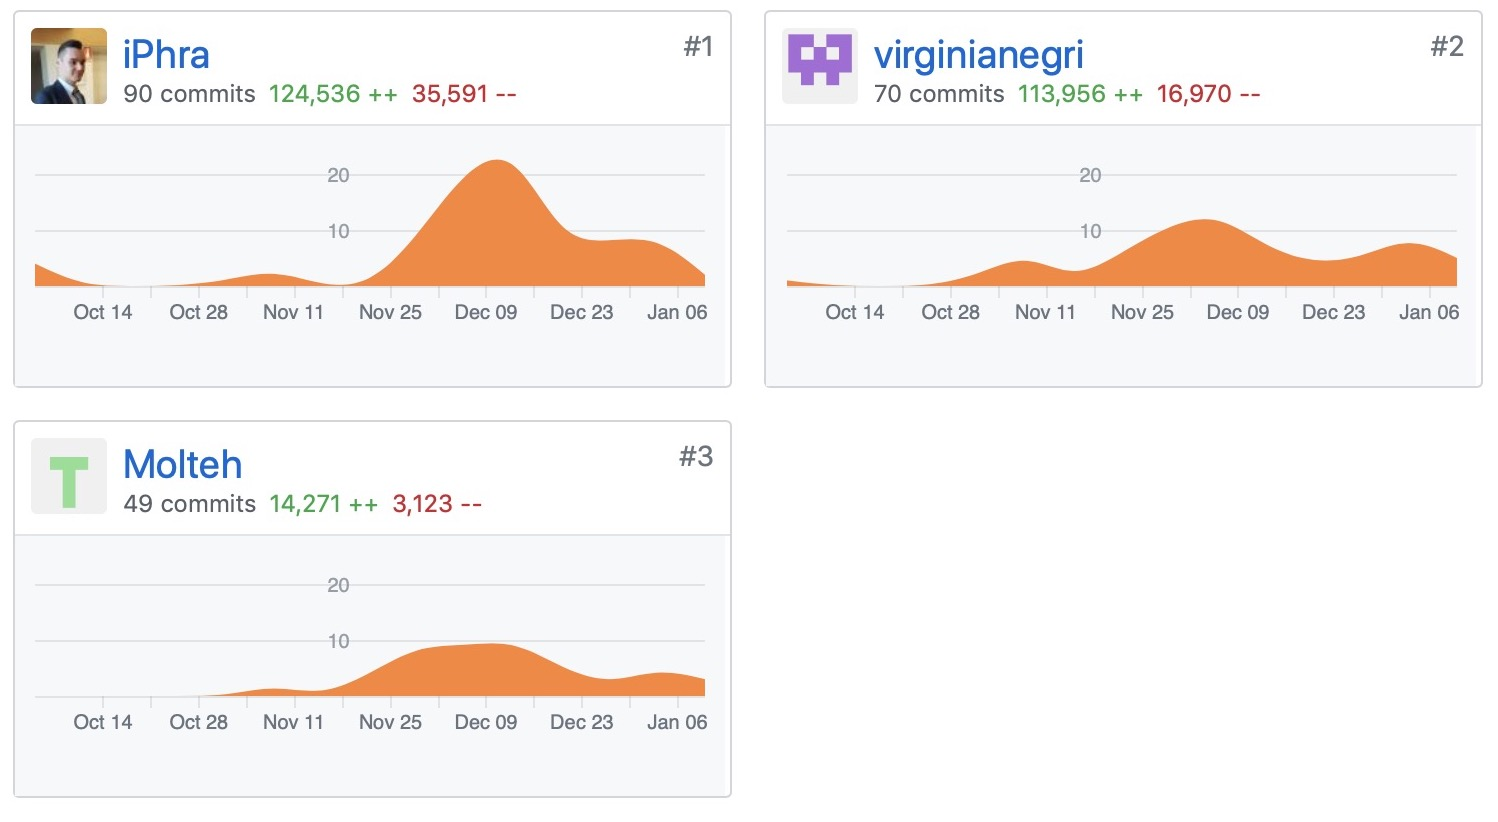
\includegraphics[width=6cm]{GitHub.png}
		\caption{GitHub contribution}
		\label{fig:Hist}
	\end{figure}
	
	The Implementation and Testing was divided as follows:
	\begin{itemize}
		\item {\bf Francesco Lorenzo:}
		contributed to the deployment of the RDS database, and its management afterwards.
		Implemented the Backend side, dealing with the WebStorm project, as well as performing Unit Testing and Integration Testing for it. After development he dealt with Server deployment.
		
		\item {\bf Luca Molteni:}
		contributed mainly on the development of the Frontend. Responsible for iOS application network layer, requests list tabs and settings tabs.
		
		\item {\bf Virginia Negri:} 
		contributed to the development of the Frontend. Responsible for implementing the main views, the health monitoring features including AutomatedSOS and for managing the client CoreData storage.
	\end{itemize}
	
	
\end{document}
